\chapter{Simulation Study and Model Validation}

Validating the model is done in two stages, in order of increasing difficulty.
We first feed the model data produced by exactly the process it assumes, the
\emph{ideal} (well-specified) data-generating process, and ask whether the
inference returns the truth; this is the subject of the first part of this chapter.
Only afterwards do we expose the model to synthetic data from ProCESS, a
cancer-evolution simulator.

\section{Simulation under the Ideal Data-Generating Process and Robustness Check}

Every experiment in this section draws its data from a single generative process
that mirrors the random-walk model of Section~\ref{sec: model rw} exactly: clone
growth rates follow a log-scale random walk along the tree, event times are placed
by stick-breaking, somatic mutations are Poisson distributed with intensity
proportional to the clone-specific molecular clock, and clone abundances are drawn
from a negative-binomial distribution on the simplex of terminal masses. Because
the data come from the model itself, any failure to recover the truth must be
blamed on the inference, on identifiability, on the sampler, or simply on the
limited information carried by a single snapshot, rather than on a mismatch
between model and data. We proceed in three steps: parameter recovery, calibration
in the stronger sense of simulation-based calibration, and a set of sensitivity
checks on the prior choices and the amount of data.

\subsection{Parameter recovery under the ideal data-generating process}

The recovery experiment follows the standard template used in Bayesian workflows
\parencite{schad2021toward}. For each replicate we draw a set of true parameters
from the priors, simulate a data set conditional on them, fit the model, and
compare the posterior with the values that actually generated the data; repeating
this over many replicates sweeps the parameter space rather than testing a single
lucky configuration.

%==================== IDEAL DGP ====================
\begin{tcolorbox}[colback=white, colframe=procblue, boxrule=0.5pt, arc=2pt,
  coltitle=white, colbacktitle=procblue, fonttitle=\bfseries\large,
  title={Ideal DGP \hfill \normalfont\normalsize Nnodes=4 \ \textbar\ Nevents=6 \ \textbar\ Nequations=8}]

\begin{tcolorbox}[colback=white, colframe=procblue!55, boxrule=0.4pt, arc=1pt,
  left=3pt,right=3pt,top=3pt,bottom=3pt]
\textbf{Topology}\quad (branching, 4 clones, 0 hidden)\\[3pt]
\texttt{Clone\_A} $\longrightarrow$ \texttt{Clone\_B} $\longrightarrow$ $\big\{\,$\texttt{Clone\_C},\ \texttt{Clone\_D}$\,\big\}$
\end{tcolorbox}

\vspace{4pt}
{\small
\begin{tabular}{@{}ll@{}}
\toprule
\textbf{Clones (all sampled)} & Clone\_A,\ Clone\_B,\ Clone\_C,\ Clone\_D \\
\textbf{Stan parents}         & (0, 1, 2, 2) \\
\textbf{number\_of\_events}   & (1, 1, 2, 2) \\
\midrule
\textbf{CNAs}                 & gain on Clone\_C and on Clone\_D \\
\textbf{Segment length}       & diploid/MRCA $10$, CNA $5$ (arbitrary units) \\
\midrule
\textbf{Growth}               & per-clone, log--random-walk along the tree \\
\textbf{Growth priors}        & $\bar w\sim\mathrm{LogN}(\log 0.06,\,0.35)$,\ $\sigma_{\log w}\sim\mathrm{Exp}(1)$,\ $\omega\sim\mathrm{LogN}(\log 1.25,\,0.5)$ \\
\textbf{Event times}          & nested-uniform stick-breaking, prior on $[0,1]$ \\
\textbf{Mutations}            & $m\sim\mathrm{Poisson}(\nu\,\mu\,\Delta t\,\ell\,c)$,\ $\mu=3$ \\
\textbf{Abundances}           & $N_i\sim\mathrm{NegBin}(N\,p_i,\,\varphi)$,\ $\varphi=100$ \\
\textbf{Equal rates}          & none (distinct by construction) \\
\bottomrule
\end{tabular}}
\end{tcolorbox}

The replicate shown below is one such draw from the process summarised in the card
above. Its four clones grow at rates $w_A=0.081$, $w_B=0.381$, $w_C=0.133$,
$w_D=0.701$ and are born at pseudotimes $0.21$, $0.80$, $0.97$, $0.88$ (clones
$A$--$D$; real times $14.1$, $25.9$, $29.4$, $27.7$ on the $[t_0,T_f]=[10,30]$ axis),
with the two copy-number events at $t=0.91$ and $t=0.85$. The simulated sample holds
$2526$ cells, split unevenly across the clones ($658$, $301$, $333$ and $1234$
for $A$--$D$): even the ideal process yields skewed clone proportions.

Figures~\ref{fig:dgp-times} and~\ref{fig:dgp-growth} show, for this representative
replicate, the posterior of the event times and of the clone growth rates against
the values that generated the data. The event-time posteriors concentrate tightly
around the truth, with the true value sitting inside the shaded $95\%$ credible
interval for every event. The growth-rate posteriors are visibly wider and more
skewed, especially for the faster-growing clones: the model still covers the truth,
but it reports this through broad intervals rather than sharp point estimates, the
first sign of the single-snapshot identifiability limit discussed below.

\begin{figure}[H]
\centering
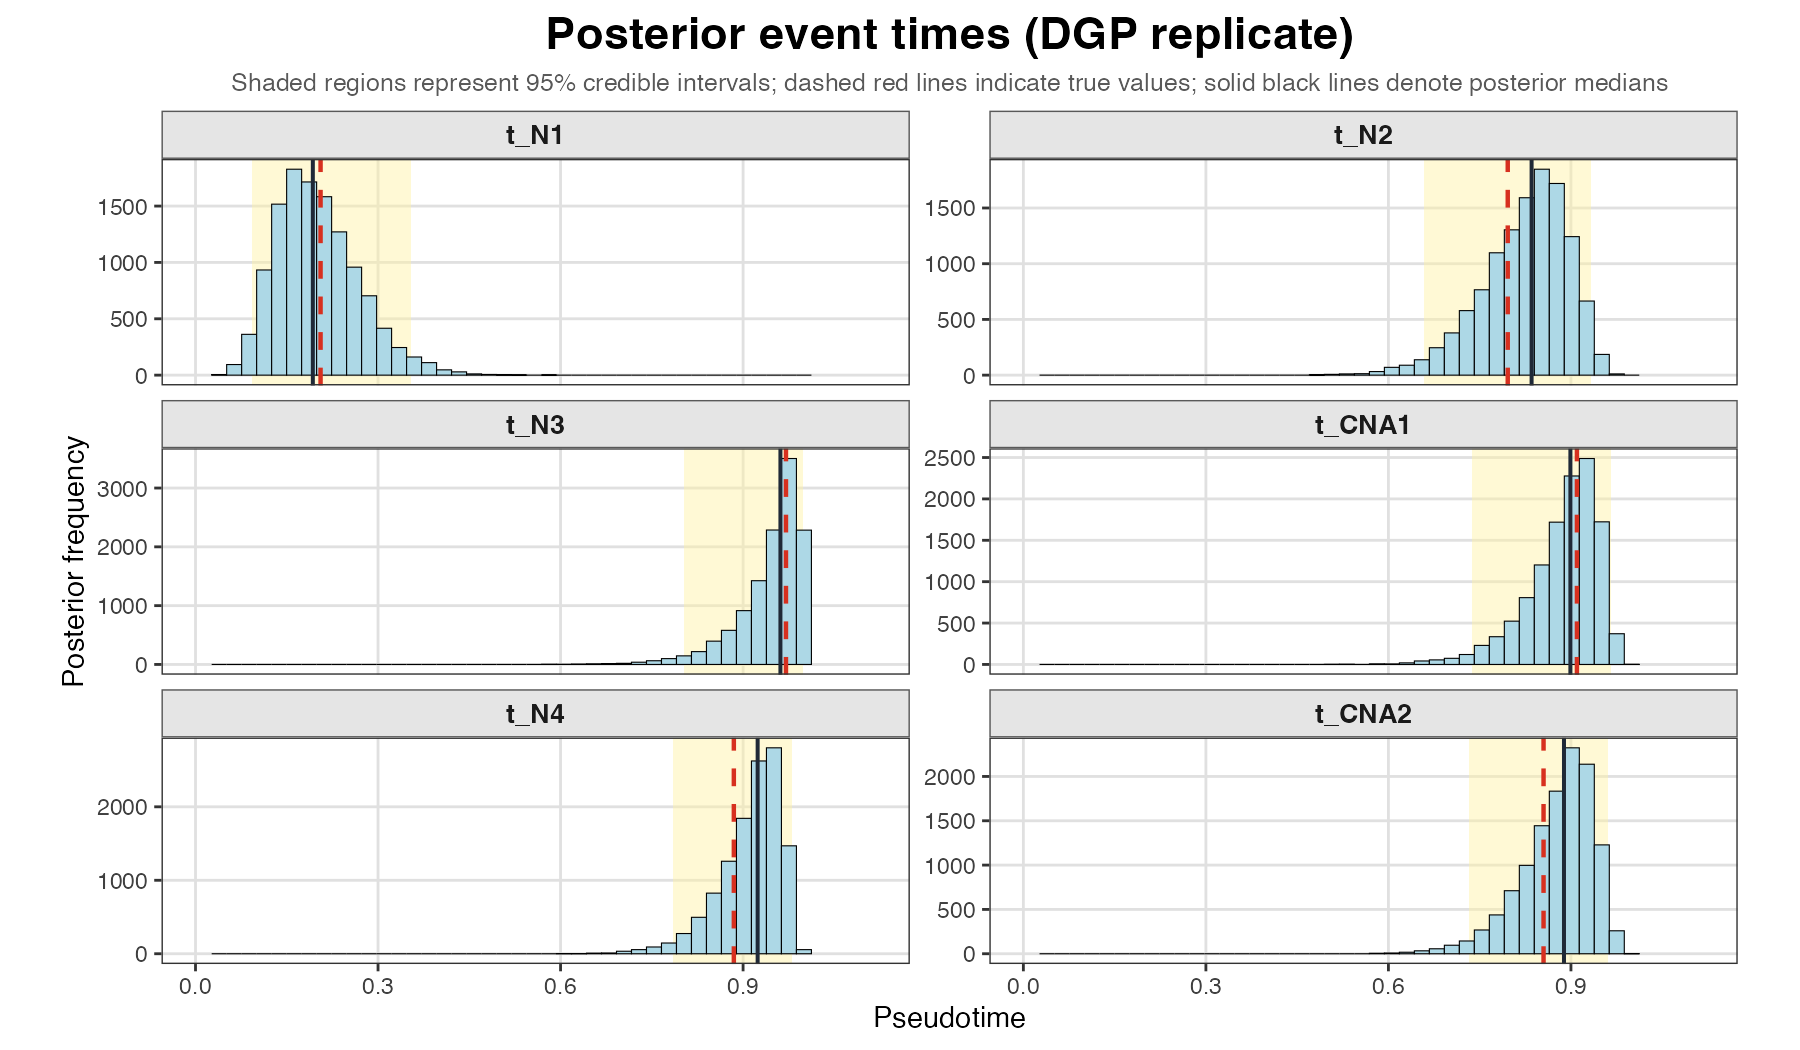
\includegraphics[width=\linewidth]{immagini/dgp_posterior_times.png}
\captionsetup{font=footnotesize}
\caption{Posterior event times for a representative replicate simulated under the
ideal data-generating process. Shaded regions are $95\%$ credible intervals, the
dashed red lines mark the true values, and the solid lines the posterior medians.}
\label{fig:dgp-times}
\end{figure}

\begin{figure}[H]
\centering
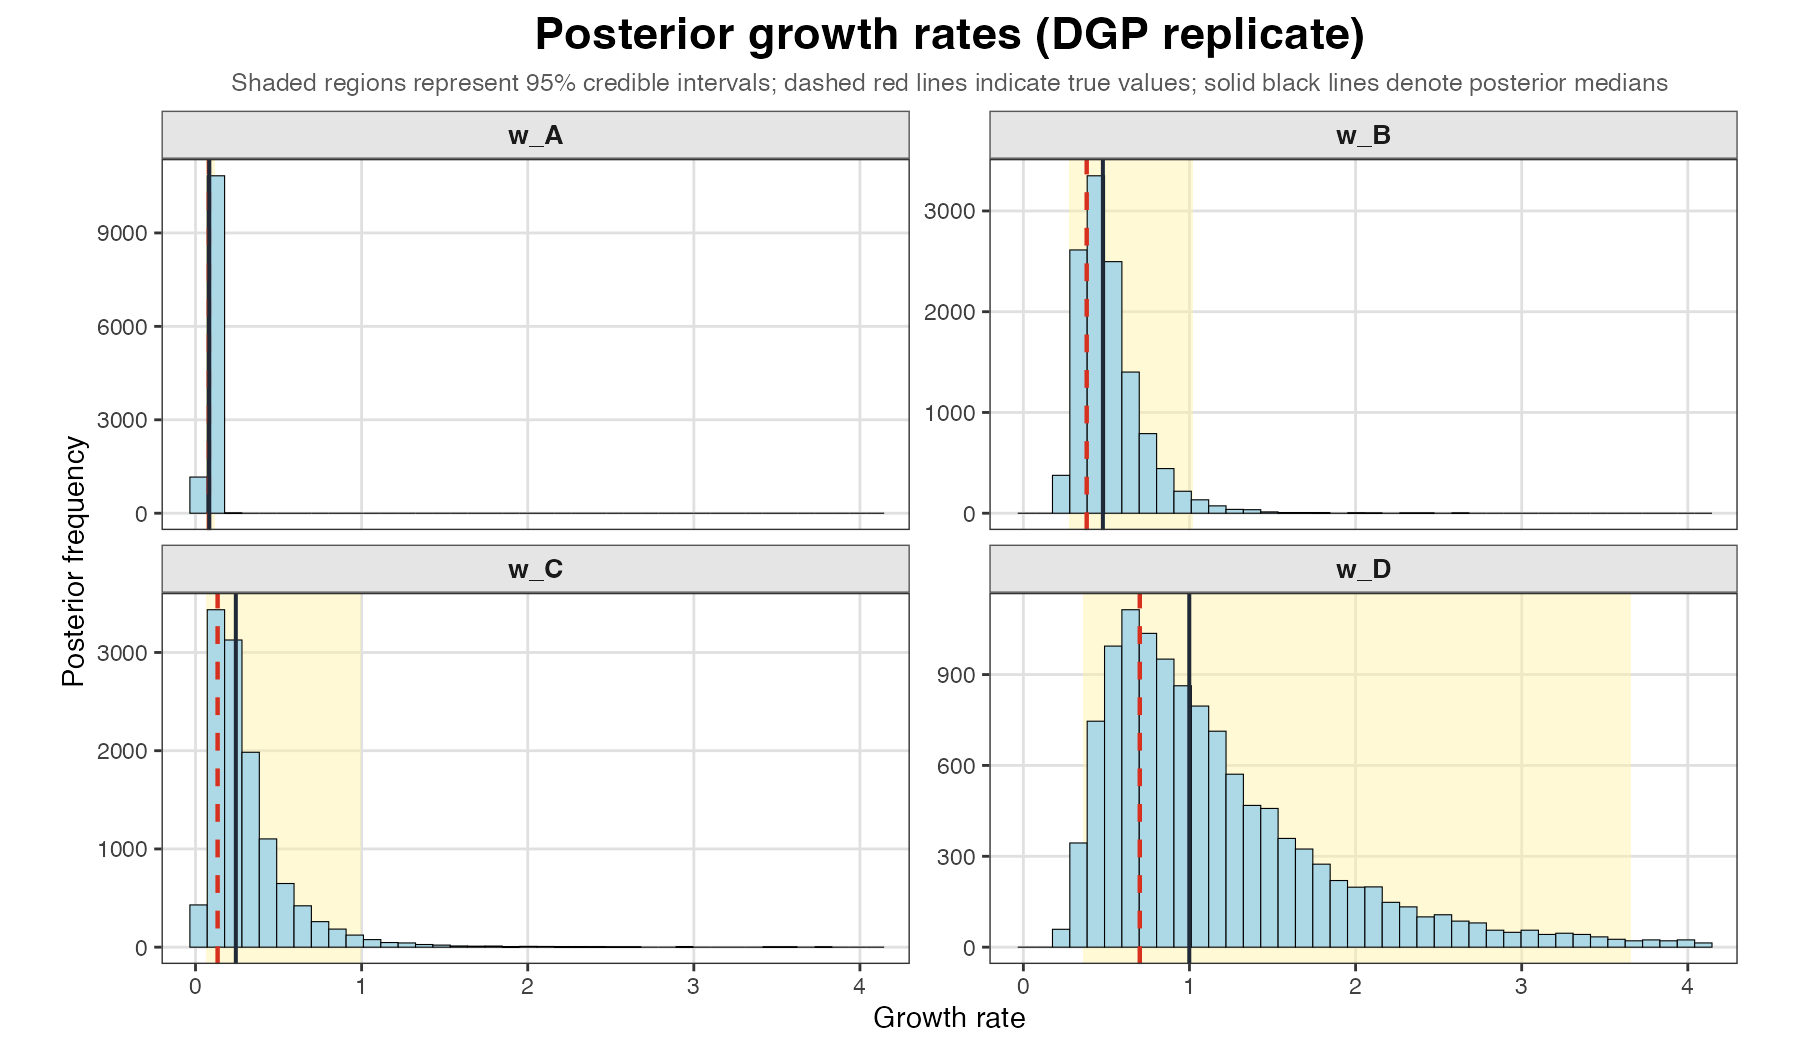
\includegraphics[width=\linewidth]{immagini/dgp_posterior_growth.png}
\captionsetup{font=footnotesize}
\caption{Posterior clone growth rates for the same replicate; conventions as in
Figure~\ref{fig:dgp-times}. The intervals are wider than for the event times,
reflecting the weaker identifiability of per-clone growth from a single snapshot.}
\label{fig:dgp-growth}
\end{figure}

A third view completes the picture. The mutation counts are the data the model
conditions on, so their posterior-predictive distribution (the
\texttt{mutations\_rep} replicates of Appendix~\ref{app: STAN 2}) measures whether
the fit can reproduce what it was given. Figure~\ref{fig:dgp-mut} shows, for the
same replicate, the predictive distribution of each of the eight mutation equations
with the observed count overlaid. Every observed value lies inside its $95\%$
posterior-predictive interval, and the predictive medians track the observations
closely across counts that range from a single mutation to several dozen: the
likelihood reproduces the data it was conditioned on, as it should under the ideal
process.

\begin{figure}[H]
\centering
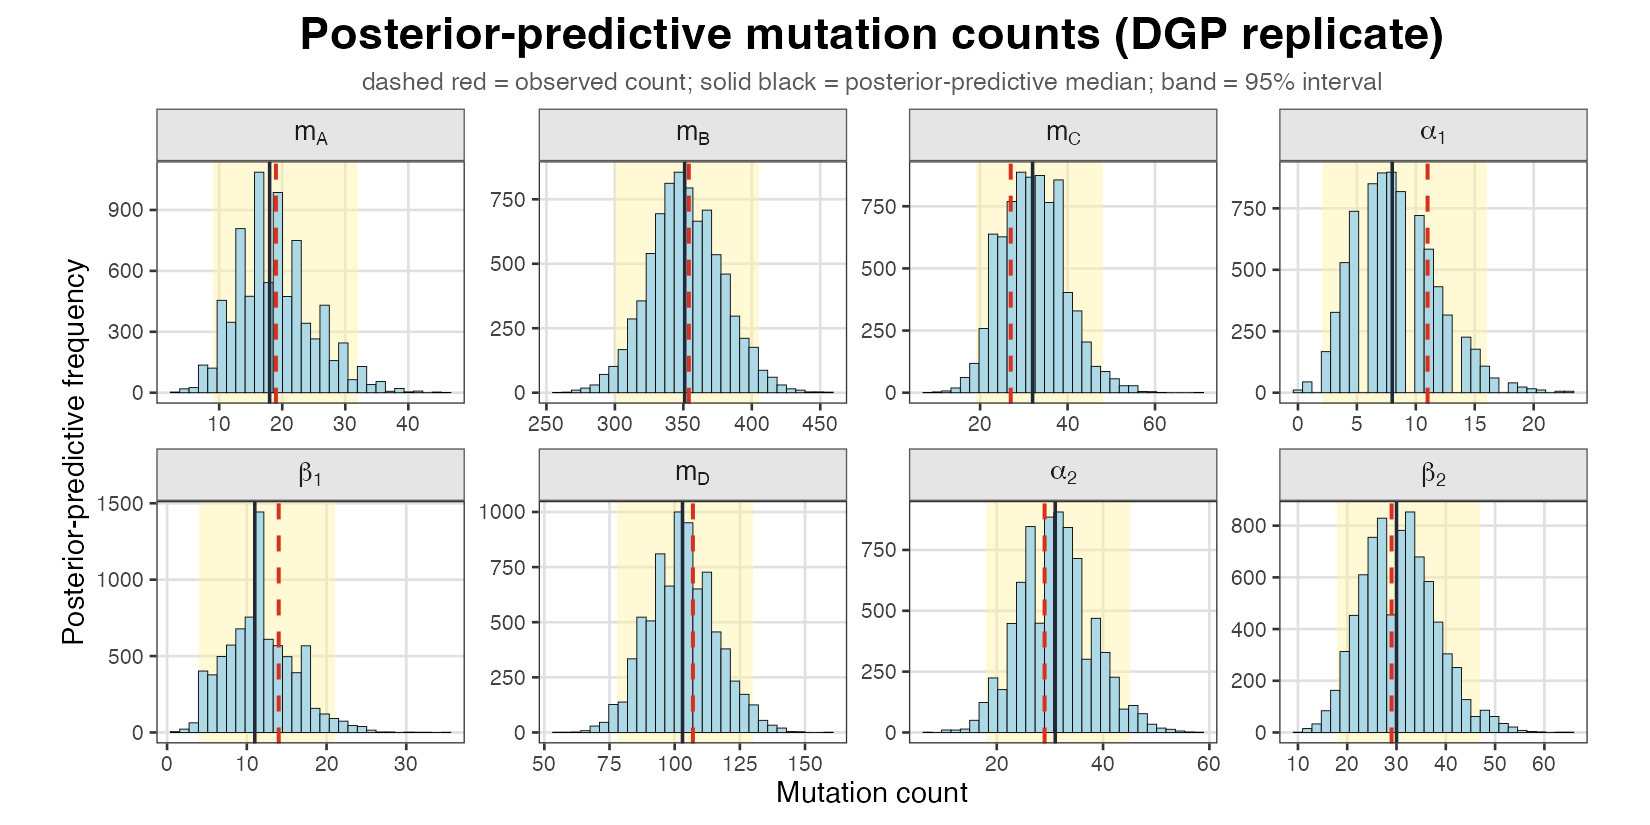
\includegraphics[width=\linewidth]{immagini/dgp_posterior_mutations.png}
\captionsetup{font=footnotesize}
\caption{Posterior-predictive distribution of the mutation counts for the same DGP
replicate. Each panel is one mutation equation; the dashed red line is the observed
count, the solid line the predictive median, and the shaded band the $95\%$
posterior-predictive interval. All eight observed counts fall inside their
intervals.}
\label{fig:dgp-mut}
\end{figure}

For this replicate the three checks agree: event times and growth rates fall within
their credible intervals, and the mutation counts are reproduced. The model behaves as
it should when the data come from its own assumptions.

This pattern holds in aggregate over the $95$ of $100$ replicates that converged.
The event times are recovered accurately and their credible intervals are well
calibrated: the mean absolute error is about $6\%$ of the $[t_0,T_f]$ window, and
the true time lies inside the $95\%$ credible interval in $97\%$ of cases, essentially
the nominal rate. The clone growth rates are a different case. Their point estimates
carry a sizeable relative error, around $23\%$, yet their intervals stay calibrated,
covering the truth in about $97\%$ of replicates: faced with a quantity it cannot pin
down, the model does not become over-confident but widens the intervals instead. This is the single-snapshot
identifiability limit: one time point constrains the \emph{product} of a clone's
growth rate and its elapsed time much better than either factor on its own, so the
model can stay calibrated even where it cannot identify the point value. The simulation-based
calibration of the next section reaches the same verdict more formally; exposing
this floor here, under ideal conditions, also sets a realistic expectation against
which the ProCESS results later in the chapter should be judged.

\subsection{Simulation-based calibration}

Recovering the truth on average is reassuring, but it is not the same thing as the
posterior being \emph{calibrated}. Calibration is a statement about frequencies:
if the model is correct, a $95\%$ credible interval should contain the true value
in $95\%$ of repeated data sets. A single fit cannot speak to this, since its
interval either covers the truth or it does not; calibration can only be judged by
simulating many data sets and aggregating.

Simulation-based calibration (SBC) turns this idea into a concrete diagnostic
\parencite{talts2018validating}, building on the posterior-quantile validation of
\textcite{cook2006validation} and later refined by \textcite{modrak2023simulation}.
The argument rests on a simple invariance. If a parameter is drawn from the prior
and a data set is then simulated from it, the true parameter is, a priori, nothing
more than one additional draw from the posterior. Its \emph{rank} among the
posterior draws is therefore uniformly distributed over its possible values.

Formally, let $\theta$ collect all model parameters (the event times, the clone
growth rates, and the global scalars $\bar w$, $\sigma_{\log w}$ and $\omega$) and
let $y$ denote the observed counts. Write the prior as $\pi(\theta)$, the likelihood
as $\pi(y\mid\theta)$ and the posterior as $\pi(\theta\mid y)$. A central object here
is the \emph{prior predictive} distribution, the distribution of the data sets the
model produces before any observation is seen: one first draws a parameter from the
prior, $\tilde\theta\sim\pi(\theta)$, and then a data set from the likelihood,
$y\sim\pi(y\mid\tilde\theta)$, so that
$\pi(y)=\int\pi(y\mid\tilde\theta)\,\pi(\tilde\theta)\,\mathrm{d}\tilde\theta$. The
method then rests on a single exact identity: averaging the \emph{posterior} over the
prior predictive returns the prior,
%
\begin{equation}
  \pi(\theta) \;=\; \iint
  \underbrace{\pi(\theta\mid y)}_{\text{posterior}}\;
  \underbrace{\pi(y\mid\tilde\theta)\,\pi(\tilde\theta)}_{\text{prior predictive}}\,
  \mathrm{d}y\,\mathrm{d}\tilde\theta .
  \label{eq:sbc-selfconsistency}
\end{equation}
%
In words: if we generate a data set from the prior predictive and then compute the
posterior it induces, the parameters we recover are distributed exactly as the prior.
The true value $\tilde\theta$ that generated the data is therefore statistically
indistinguishable from an ordinary draw of that posterior.
%
A single SBC iteration draws a ground truth from the prior, simulates a data set
from it, and fits the model,
%
\begin{equation}
  \tilde\theta \sim \pi(\theta), \qquad
  \tilde y \sim \pi(y\mid\tilde\theta), \qquad
  \theta_1,\dots,\theta_L \sim \pi(\theta\mid\tilde y),
  \label{eq:sbc-generative}
\end{equation}
%
and, for any one-dimensional summary $f$ of the parameters (here simply each
parameter in turn), records the \emph{rank} of the true value among the $L$ posterior
draws. The rank is just the count of how many posterior draws fall below the true
value: a whole number between $0$, when the truth is smaller than every draw, and $L$,
when it is larger than all of them,
%
\begin{equation}
  r \;=\; \sum_{\ell=1}^{L} \mathbf{1}\!\left[\, f(\theta_\ell) < f(\tilde\theta) \,\right]
  \;\in\; \{0,1,\dots,L\},
  \label{eq:sbc-rank}
\end{equation}
%
where $\mathbf{1}[\cdot]$ is the indicator that equals $1$ when its condition holds
and $0$ otherwise.
Whenever the posterior is computed exactly, this rank is uniformly distributed; this
is the result that turns SBC into a calibration test.

\begin{theorem}[Rank uniformity under calibration]
\label{thm:sbc}
Let $\tilde\theta\sim\pi(\theta)$ and $\tilde y\sim\pi(y\mid\tilde\theta)$, and let
$\theta_1,\dots,\theta_L$ be independent draws from the exact posterior
$\pi(\theta\mid\tilde y)$. For any one-dimensional summary $f$, the rank $r$ of
equation~\eqref{eq:sbc-rank} satisfies
\begin{equation}
  r \sim \operatorname{Uniform}\{0,1,\dots,L\}.
  \label{eq:sbc-uniform}
\end{equation}
\end{theorem}

\begin{proof}
By the self-consistency identity~\eqref{eq:sbc-selfconsistency} every posterior draw
$\theta_\ell$ shares the marginal distribution $\pi(\theta)$ of $\tilde\theta$. The
$L+1$ values $(\tilde\theta,\theta_1,\dots,\theta_L)$ are therefore exchangeable, so
$\tilde\theta$ is equally likely to occupy any of the $L+1$ order positions among the
draws, and its rank is uniform on $\{0,\dots,L\}$.
\end{proof}

In the limit $L\to\infty$ the normalised rank converges to the
posterior quantile of the true value,
%
\begin{equation}
  \frac{r}{L} \;\xrightarrow{\;L\to\infty\;}\;
  u \;=\; \Pr_{\theta\sim\pi(\cdot\mid\tilde y)}\!\left[\, f(\theta) < f(\tilde\theta) \,\right],
  \qquad u \sim \operatorname{Uniform}(0,1),
  \label{eq:sbc-pit}
\end{equation}
%
which is the posterior-quantile criterion of
\textcite{cook2006validation}; simulation-based calibration is its discrete,
rank-based and Markov-chain-robust counterpart.

Over $N$ independent iterations the ranks are collected into a histogram of $B$
bins. Each iteration contributes exactly one rank, and under~\eqref{eq:sbc-uniform}
that rank is equally likely to land in any of the $B$ bins, independently of the
others. The count $c_b$ in a given bin is therefore a sum of $N$ independent
Bernoulli trials, each a success (the rank landing in bin $b$) with probability
$1/B$, which is by definition a binomial,
%
\begin{equation}
  c_b \sim \operatorname{Binomial}\!\left(N, \tfrac{1}{B}\right), \qquad
  \mathbb{E}[c_b] = \frac{N}{B},
  \label{eq:sbc-bins}
\end{equation}
%
so every bar should sit at the same expected height $N/B$ up to binomial sampling
noise, and a flat histogram lying inside the band
$\big[\operatorname{qbinom}(\tfrac{\alpha}{2},N,\tfrac1B),\,
\operatorname{qbinom}(1-\tfrac{\alpha}{2},N,\tfrac1B)\big]$ (with $\alpha=0.01$,
the grey band of Figure~\ref{fig:sbc}) is consistent with calibration.
Characteristic departures instead diagnose specific failures: a $\cup$ shape, with
mass piling at the two extremes $0$ and $L$, signals posteriors that are too
\emph{narrow} (over-confident), because the true value then falls in the tails; a
$\cap$ shape, with mass in the centre, signals posteriors that are too \emph{wide}
(under-confident); and a monotone slope signals a location bias. Two practical
points matter. First, because Markov-chain draws are autocorrelated, the $L$
retained draws are thinned until approximately independent, as otherwise the ranks
depart from uniformity even for an exact posterior. Second, the prior used to
generate the data must coincide \emph{exactly} with the one used to fit; the
refinement of \textcite{modrak2023simulation} shows, moreover, that augmenting the
parameters with data-dependent test quantities makes the check sensitive to
failure modes that the parameter ranks alone can miss.

We ran SBC on the same model and tree. As the method requires, and unlike the
recovery experiment above, the ground truth here is drawn from the \emph{exact}
model prior, with no clamping, so that the prior used to generate the data and the
prior used to fit it coincide; replicates that failed to converge are discarded,
since the rank of a non-converged chain is meaningless. Figure~\ref{fig:sbc} shows
the resulting rank histograms, one per parameter, with the grey band giving the
$99\%$ interval expected under uniformity. Of the $1000$ simulations, $966$ converged
and were retained.\footnote{A small fraction of transitions (around $2\%$ on
average) ended in divergences; since every retained fit satisfied $\hat R<1.1$ this
does not affect the rank statistics, although it suggests that a higher
\texttt{adapt\_delta} would be prudent in production runs.}
Across the board the histograms are consistent with uniformity. For the global
parameters ($\bar w$, $\sigma_{\log w}$, $\omega$) and for the six event times the
bars scatter around the expected level with no systematic $\cup$, $\cap$ or sloped
pattern, so the corresponding posteriors are neither over- nor under-confident and
show no detectable bias. The per-clone growth histograms ($w_{\mathrm{node}}$) are
visibly noisier, and one or two bins reach the edge of the band. This is about what
one would expect by chance from the roughly $280$ bins inspected at the $99\%$ level,
and is unsurprising given the weaker identifiability of growth; the histograms still
show no coherent departure from uniformity. Together with the recovery experiment,
this is evidence that the sampler and the model implementation are faithful and that
the uncertainties the model reports are calibrated.

\begin{figure}[H]
\centering
\IfFileExists{immagini/sbc_rank_histograms.png}
  {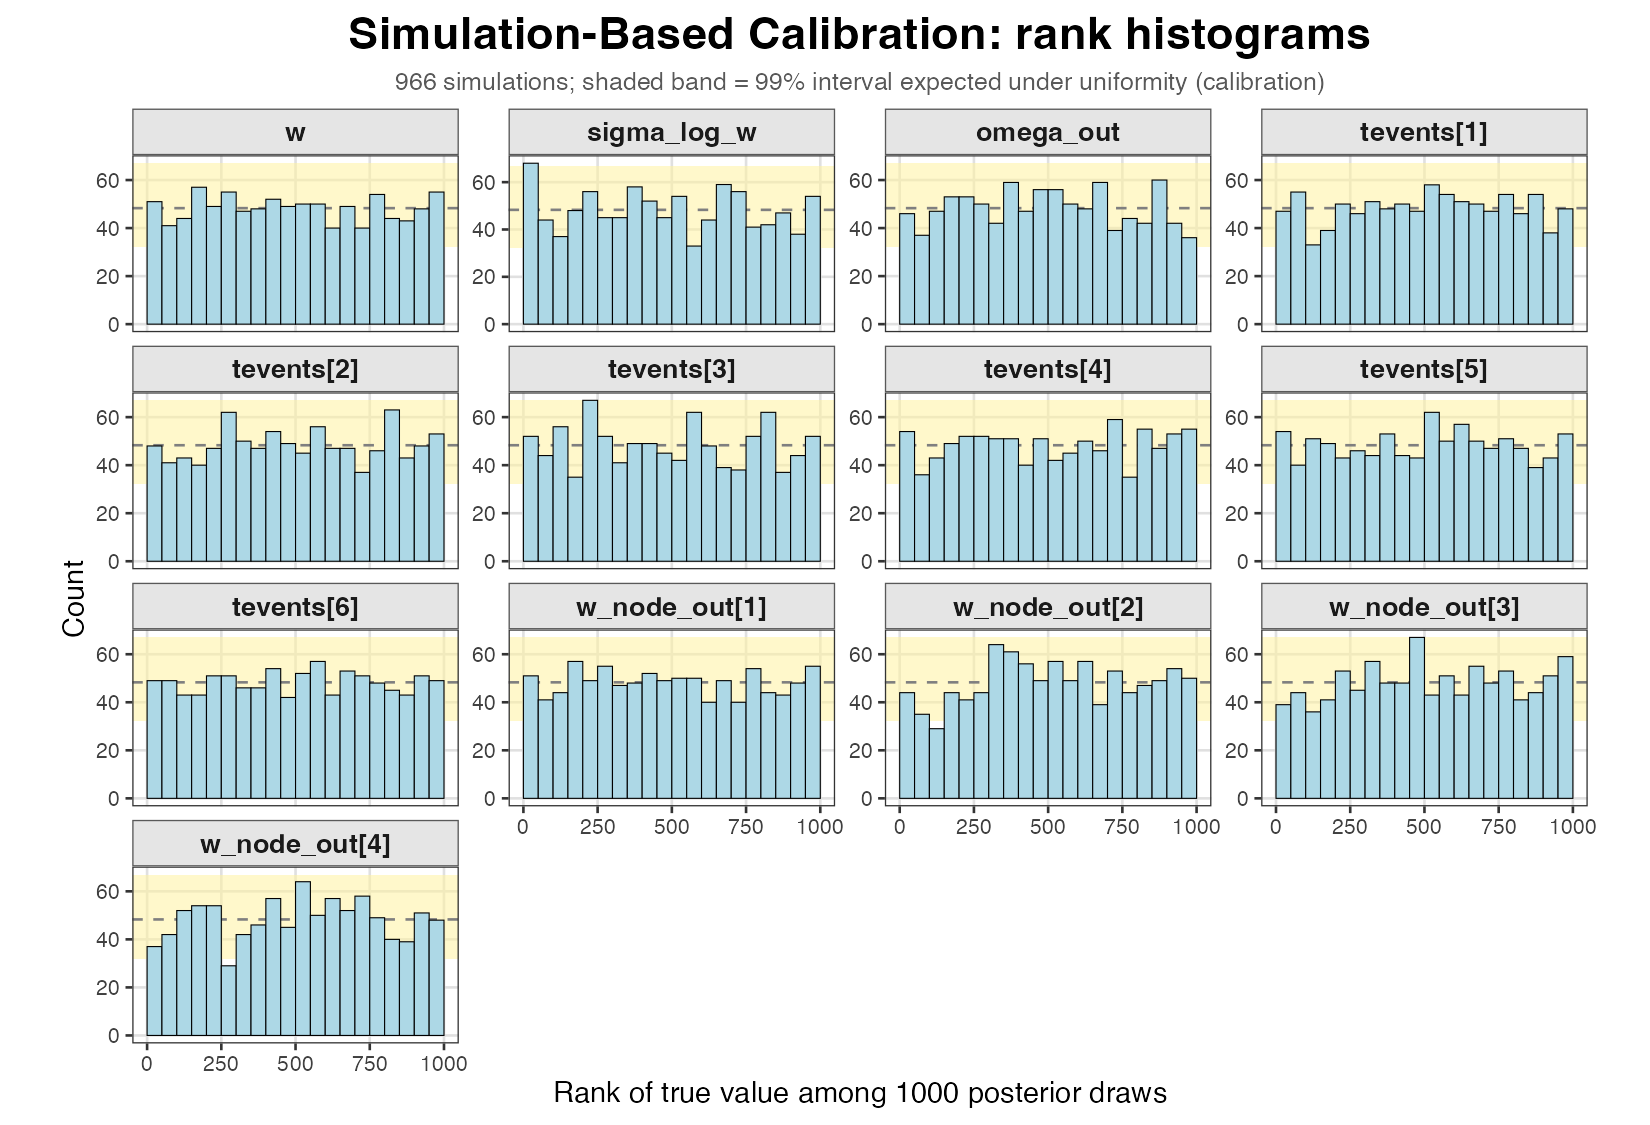
\includegraphics[width=\linewidth]{immagini/sbc_rank_histograms.png}}
  {\fbox{\parbox{0.82\linewidth}{\centering\vspace{2.2cm}\itshape Generate this
   figure by running \texttt{robustness\_checks/06\_sbc.R}\\(produces
   \texttt{immagini/sbc\_rank\_histograms.png}).\vspace{2.2cm}}}}
\captionsetup{font=footnotesize}
\caption{Simulation-based calibration: rank of the true value among the (thinned)
posterior draws, aggregated over simulations, for each model parameter. Under a
calibrated inference the ranks are uniform; the grey band is the $99\%$ interval
expected under uniformity. A $\cup$ shape would indicate over-confidence
(intervals too narrow), a $\cap$ shape under-confidence (too wide), and a slope a
bias.}
\label{fig:sbc}
\end{figure}

\subsection{Robustness checks}

A trustworthy inference should not hinge on choices the analyst makes somewhat
arbitrarily, nor collapse when the data grow scarcer. The robustness checks probe
exactly this: we vary, one quantity at a time, the inputs the model is most exposed
to, and watch whether the recovery of the event times holds up. Four sweeps are run
under the ideal DGP, testing the quantities most open to question:
%
\begin{itemize}
  \item the width of the prior on the clock-to-growth factor $\omega$;
  \item the rate $\lambda$ of the prior on the random-walk step $\sigma_{\log w}$;
  \item the number of sequenced cells (the sampling depth);
  \item the dispersion $\varphi$ of the negative-binomial abundance likelihood.
\end{itemize}
%
For each sweep we record, for every event, three quantities averaged over replicates:
the absolute bias (the distance of the posterior median from the truth), the $95\%$
coverage (how often the credible interval contains the truth), and the width of that
credible interval, that is the length of the $95\%$ interval, which measures how sharp
or uncertain the estimate is. A good inference keeps coverage near the nominal $0.95$
while making the width as small as the data allow; an over-tight prior, for instance,
narrows the width but at the cost of coverage. The four figures below report one sweep
each, followed by its reading.

\begin{figure}[H]
\centering
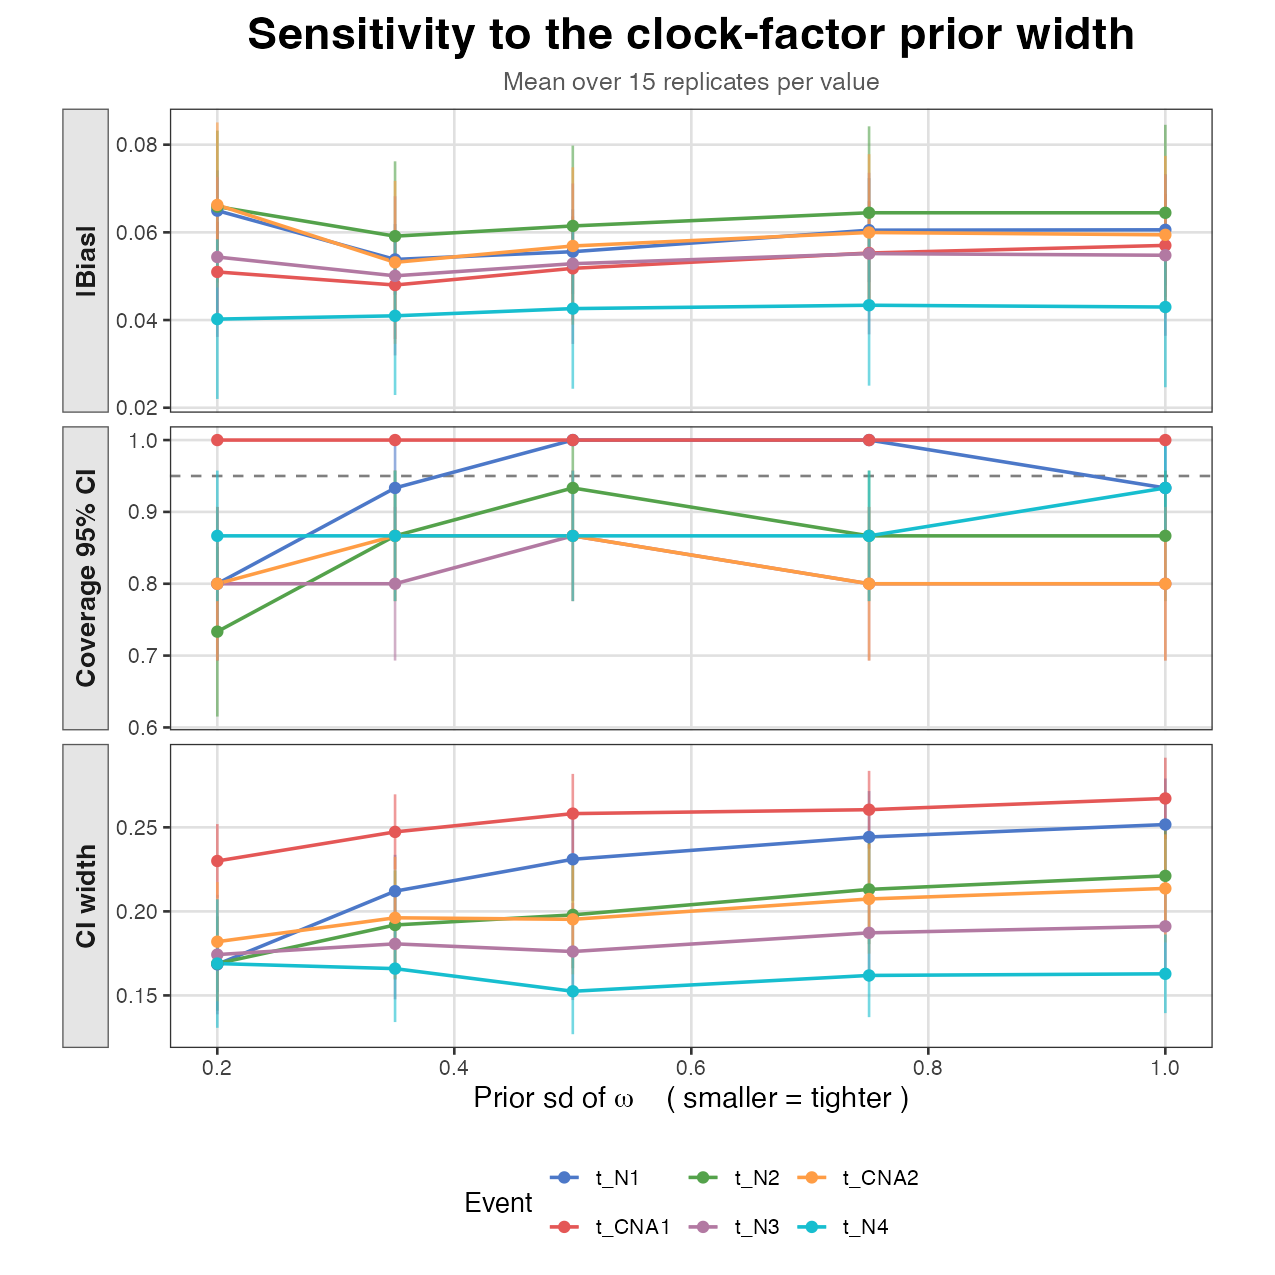
\includegraphics[width=0.74\linewidth]{immagini/robust_sweep_omega_sd.png}
\captionsetup{font=footnotesize}
\caption{Sensitivity to the width of the clock-factor prior. Per-event absolute
bias, $95\%$ coverage and credible-interval width as the prior $\mathrm{sd}$ of
$\omega$ is varied (mean over replicates; error bars are standard errors). An
over-tight prior under-covers; the dashed line marks the nominal $0.95$ coverage.}
\label{fig:sweep-omega}
\end{figure}

The width of the $\omega$ prior is the one choice that genuinely matters
(Figure~\ref{fig:sweep-omega}). An over-tight prior ($\mathrm{sd}=0.2$) yields
over-confident intervals that under-cover for several events; from about
$\mathrm{sd}=0.5$ onwards the coverage returns close to nominal, at the modest price
of slightly wider intervals.

\begin{figure}[H]
\centering
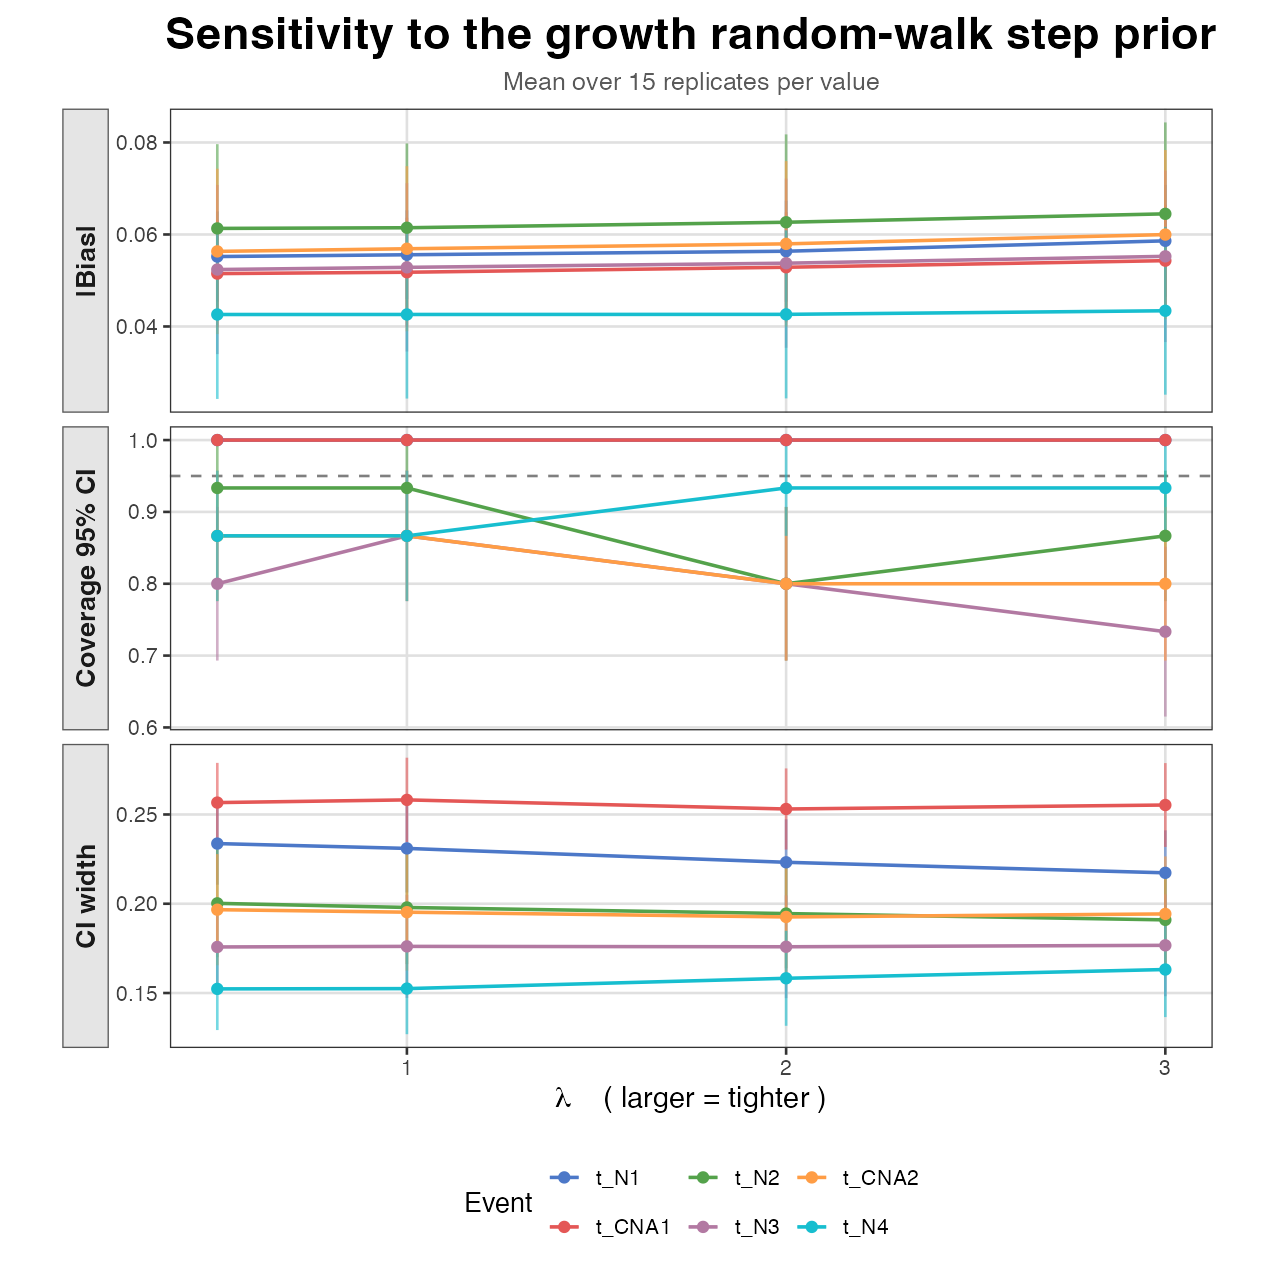
\includegraphics[width=0.74\linewidth]{immagini/robust_sweep_sigma_rate.png}
\captionsetup{font=footnotesize}
\caption{Sensitivity to the prior on the growth random-walk step,
$\sigma_{\log w}\sim\mathrm{Exponential}(\lambda)$. Bias and coverage are largely
insensitive to $\lambda$ on this topology.}
\label{fig:sweep-sigma}
\end{figure}

The prior on the growth random-walk step has a much milder effect
(Figure~\ref{fig:sweep-sigma}): on this topology bias and coverage are essentially
flat across $\lambda$, and the chosen $\lambda=1$ is the value that best balances the
competing demands of chain-like and branching trees.

\begin{figure}[H]
\centering
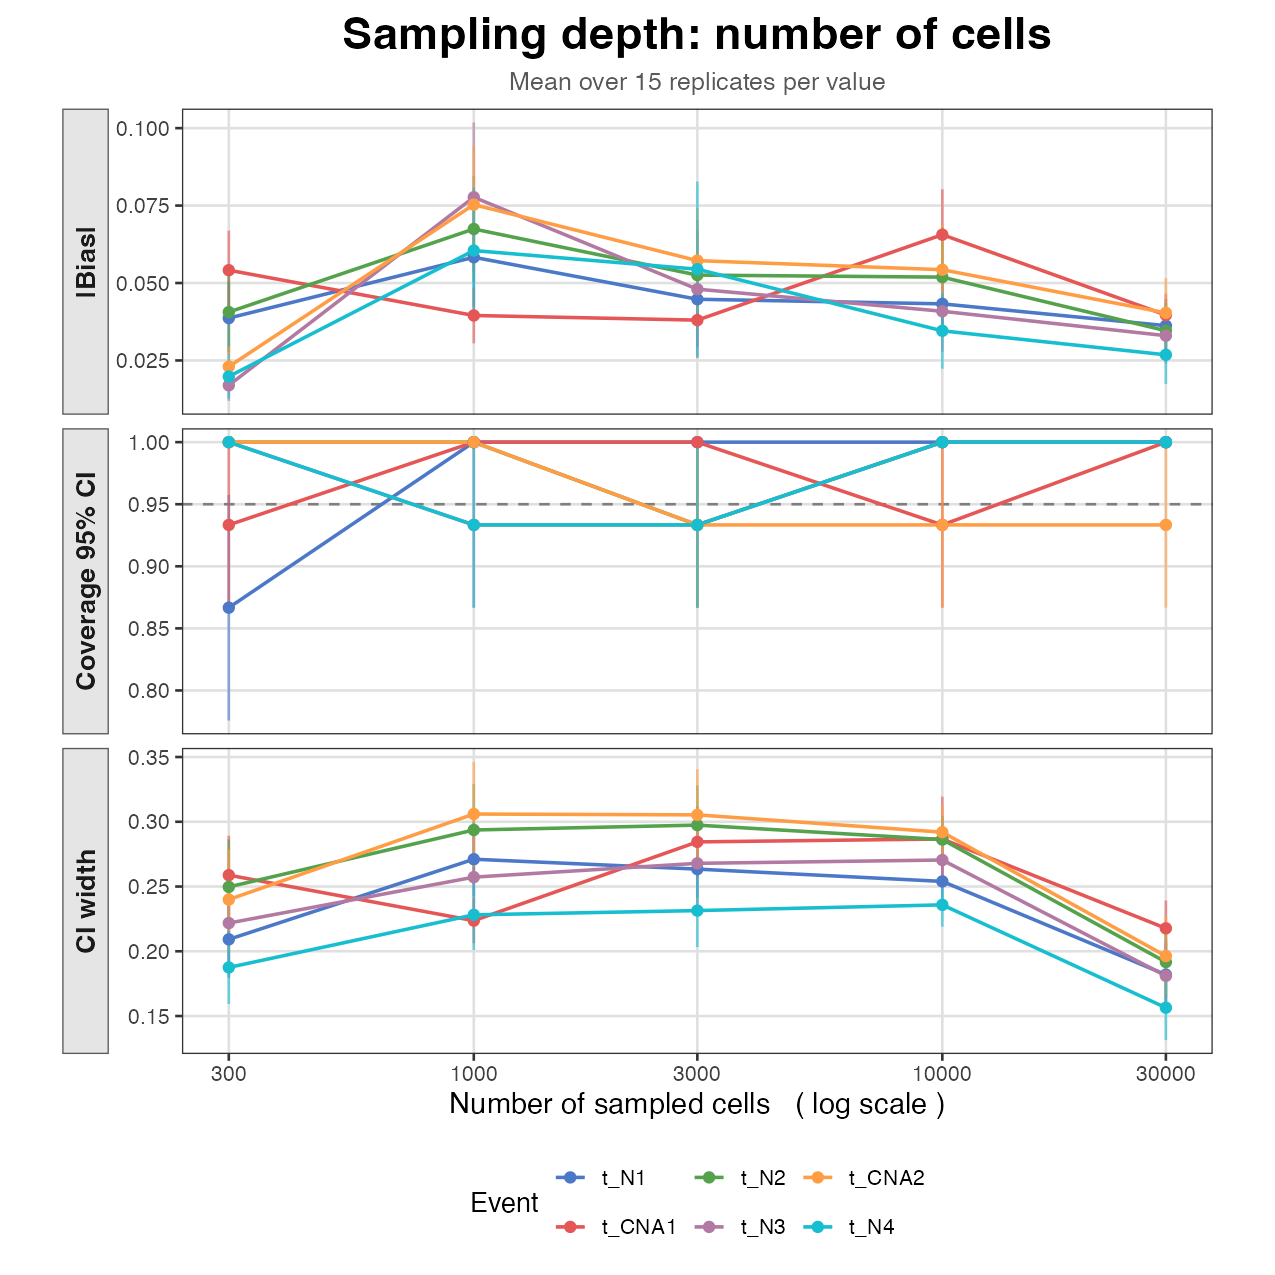
\includegraphics[width=0.74\linewidth]{immagini/robust_sweep_ncells.png}
\captionsetup{font=footnotesize}
\caption{Effect of sampling depth. As the number of sequenced cells grows, the
bias falls and the credible intervals tighten while coverage remains close to
nominal.}
\label{fig:sweep-ncells}
\end{figure}

Sampling depth behaves exactly as one would hope (Figure~\ref{fig:sweep-ncells}):
more cells lower the bias and tighten the intervals while coverage stays close to
nominal, a sign that the inference puts the extra data to good use instead of growing
overconfident.

\begin{figure}[H]
\centering
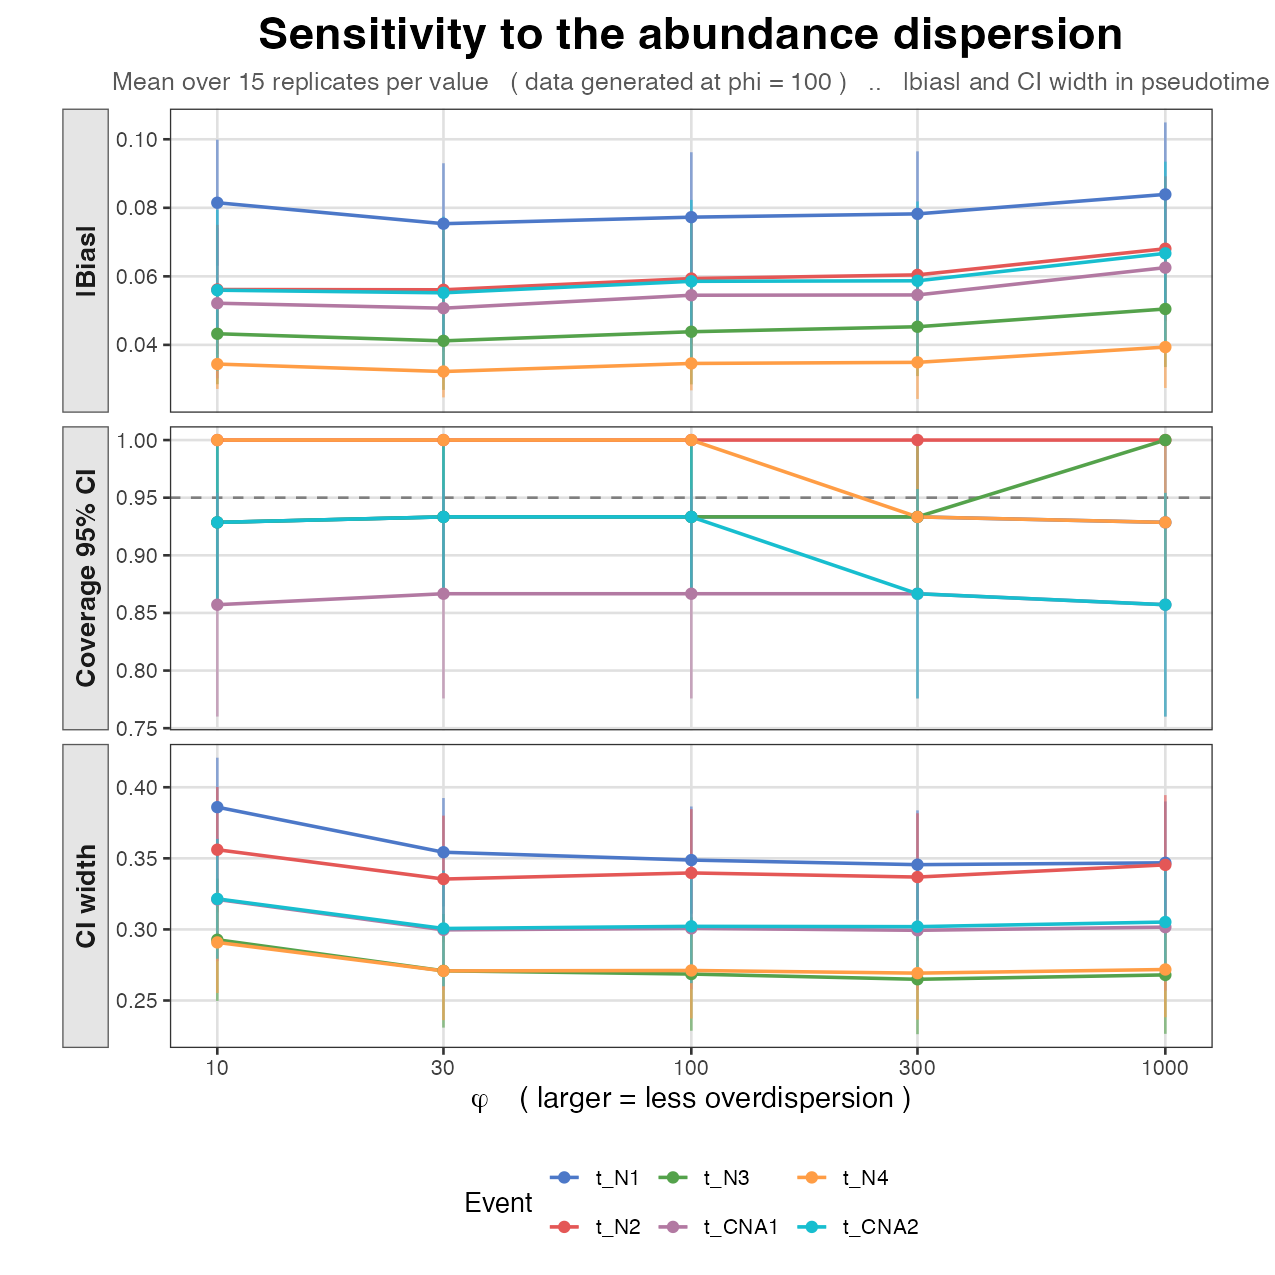
\includegraphics[width=0.74\linewidth]{immagini/robust_sweep_phi.png}
\captionsetup{font=footnotesize}
\caption{Sensitivity to the dispersion $\varphi$ of the negative-binomial abundance
likelihood (data generated at $\varphi=100$). Event-time bias and coverage are flat
across two orders of magnitude of $\varphi$; only very strong overdispersion
($\varphi=10$) widens the credible intervals.}
\label{fig:sweep-phi}
\end{figure}

The dispersion $\varphi$ of the abundance likelihood matters less still
(Figure~\ref{fig:sweep-phi}): event-time recovery barely moves as $\varphi$ ranges
over two orders of magnitude, and only at the most overdispersed setting
($\varphi=10$, the noisiest abundances) do the intervals widen a little, with bias
and coverage flat throughout. This fits the rest of the chapter: the timing is
carried by the mutation counts, so how noisy one assumes the abundances to be barely
reaches the event times.

These checks point the same way. Under its own assumptions the
model recovers event times accurately and with calibrated uncertainty, it passes
simulation-based calibration, and it is robust both to reasonable changes in the
priors and to the amount of data available. The one limitation that surfaces, the
residual uncertainty on per-clone growth, is a property of single-snapshot data
rather than a flaw in the implementation, and it sets the bar against which the
ProCESS experiments in the rest of this chapter should be judged.
\section{ProCESS: a linear four-clone tumour}

The ideal-DGP experiments show what the model can do under its own assumptions; the
real test is whether those conclusions survive when the data are produced by a
different mechanism. ProCESS is a spatial simulator of clonal tumour growth: cells
divide, mutate and acquire copy-number alterations on a two-dimensional lattice, and
a region of the final tumour is sequenced \parencite{process}.

We study two scenarios, a four-clone linear chain and a six-clone
branching tree, both sampled by a localized biopsy (\emph{DLP$^+$}): a
contiguous patch of tissue that over- and under-represents clones and so distorts the
abundance signal the model relies on. This is the regime that matters in practice,
since a real biopsy is never a proportional draw from the clone simplex; the
well-specified, proportional-like case is the one already covered by the ideal-DGP
analysis above. Any degradation seen here therefore measures robustness to a doubly
adverse setting at once: a different growth mechanism \emph{and} a distorted sample.
The two trees are summarized in the cards opening the respective sections; for each we
show the simulated tissue with the biopsied region marked, the reconstructed mutation
phylogeny, and the posteriors of the event pseudotimes, the clone growth rates and the
mutation counts against the ground truth. The bias of the event-time and growth-rate
recovery is summarised, for both scenarios, in Table~\ref{tab:sim-bias}. Event times
are on the unit pseudotime scale, $t=0$ the tumour origin and $t=1$ the moment of
sequencing.

%==================== CLONE 4 ====================
\begin{tcolorbox}[colback=white, colframe=procblue, boxrule=0.5pt, arc=2pt,
  coltitle=white, colbacktitle=procblue, fonttitle=\bfseries\large,
  title={Linear chain (4 clones) \hfill \normalfont\normalsize Nnodes=4 \ \textbar\ Nevents=6 \ \textbar\ Nequations=8}]

\begin{tcolorbox}[colback=white, colframe=procblue!55, boxrule=0.4pt, arc=1pt,
  left=3pt,right=3pt,top=3pt,bottom=3pt]
\textbf{Topology}\quad (linear, 4 sampled, 0 hidden)\\[3pt]
\texttt{Clone\_A} $\longrightarrow$ \texttt{Clone\_B} $\longrightarrow$ \texttt{Clone\_C} $\longrightarrow$ \texttt{Clone\_D}
\end{tcolorbox}

\vspace{4pt}
\begin{tabular}{@{}ll@{}}
\toprule
\textbf{Sampled}            & Clone\_A,\ Clone\_B,\ Clone\_C,\ Clone\_D \\
\textbf{Sampling}           & localized biopsy (DLP$^+$) \\
\textbf{Stan parents}       & (0, 1, 2, 3) \\
\textbf{number\_of\_events} & (2, 1, 2, 1) \\
\midrule
\textbf{CNAs}               & CNA\_A on Clone\_A -- chr12, 40\,Mb \\
                            & CNA\_C\_hidden in Clone\_C -- chr5, 20\,Mb \\
\midrule
\textbf{Growth rates}       & $w_A{=}0.0493$\quad $w_B{=}0.0983$\quad $w_C{=}0.1350$\quad $w_D{=}0.1883$ \\
\textbf{Equal rates}        & none \\
\bottomrule
\end{tabular}
\end{tcolorbox}



The localized biopsy of this tumour returned only $192$ cells, very unevenly split
across the four clones: $10$ from the founder $A$, $98$ from $B$, $47$ from $C$ and
$37$ from $D$. On the simulator's clock the tumour is sequenced at $T_f\approx 86$,
and the ground-truth births are $t_B=0.38$, $t_C=0.53$, $t_D=0.74$ in pseudotime
(real times $\approx 33$, $46$ and $64$), with the two root-clone events pinned at
the origin. The clone growth rates and copy-number events are those listed in the
card above; the recovered quantities are collected in Table~\ref{tab:sim-bias}.

The four-clone chain is the gentler of the two trees. The biopsy
(Figure~\ref{fig:c4d-sampled}) over- and under-represents the clones, yet the
inference holds up. The event pseudotimes are recovered with a mean absolute error of
$0.020$, the only two events left uncovered being those on the root clone~A, whose
true time is essentially zero: pinned against the boundary $t=0$, a strictly positive
posterior cannot quite reach them, so these are boundary artefacts rather than genuine
misses (Figure~\ref{fig:c4d-times}). The growth rates are recovered to about $11\%$
with all four intervals covering the truth (Figure~\ref{fig:c4d-growth}).

\begin{figure}[H]
    \centering
    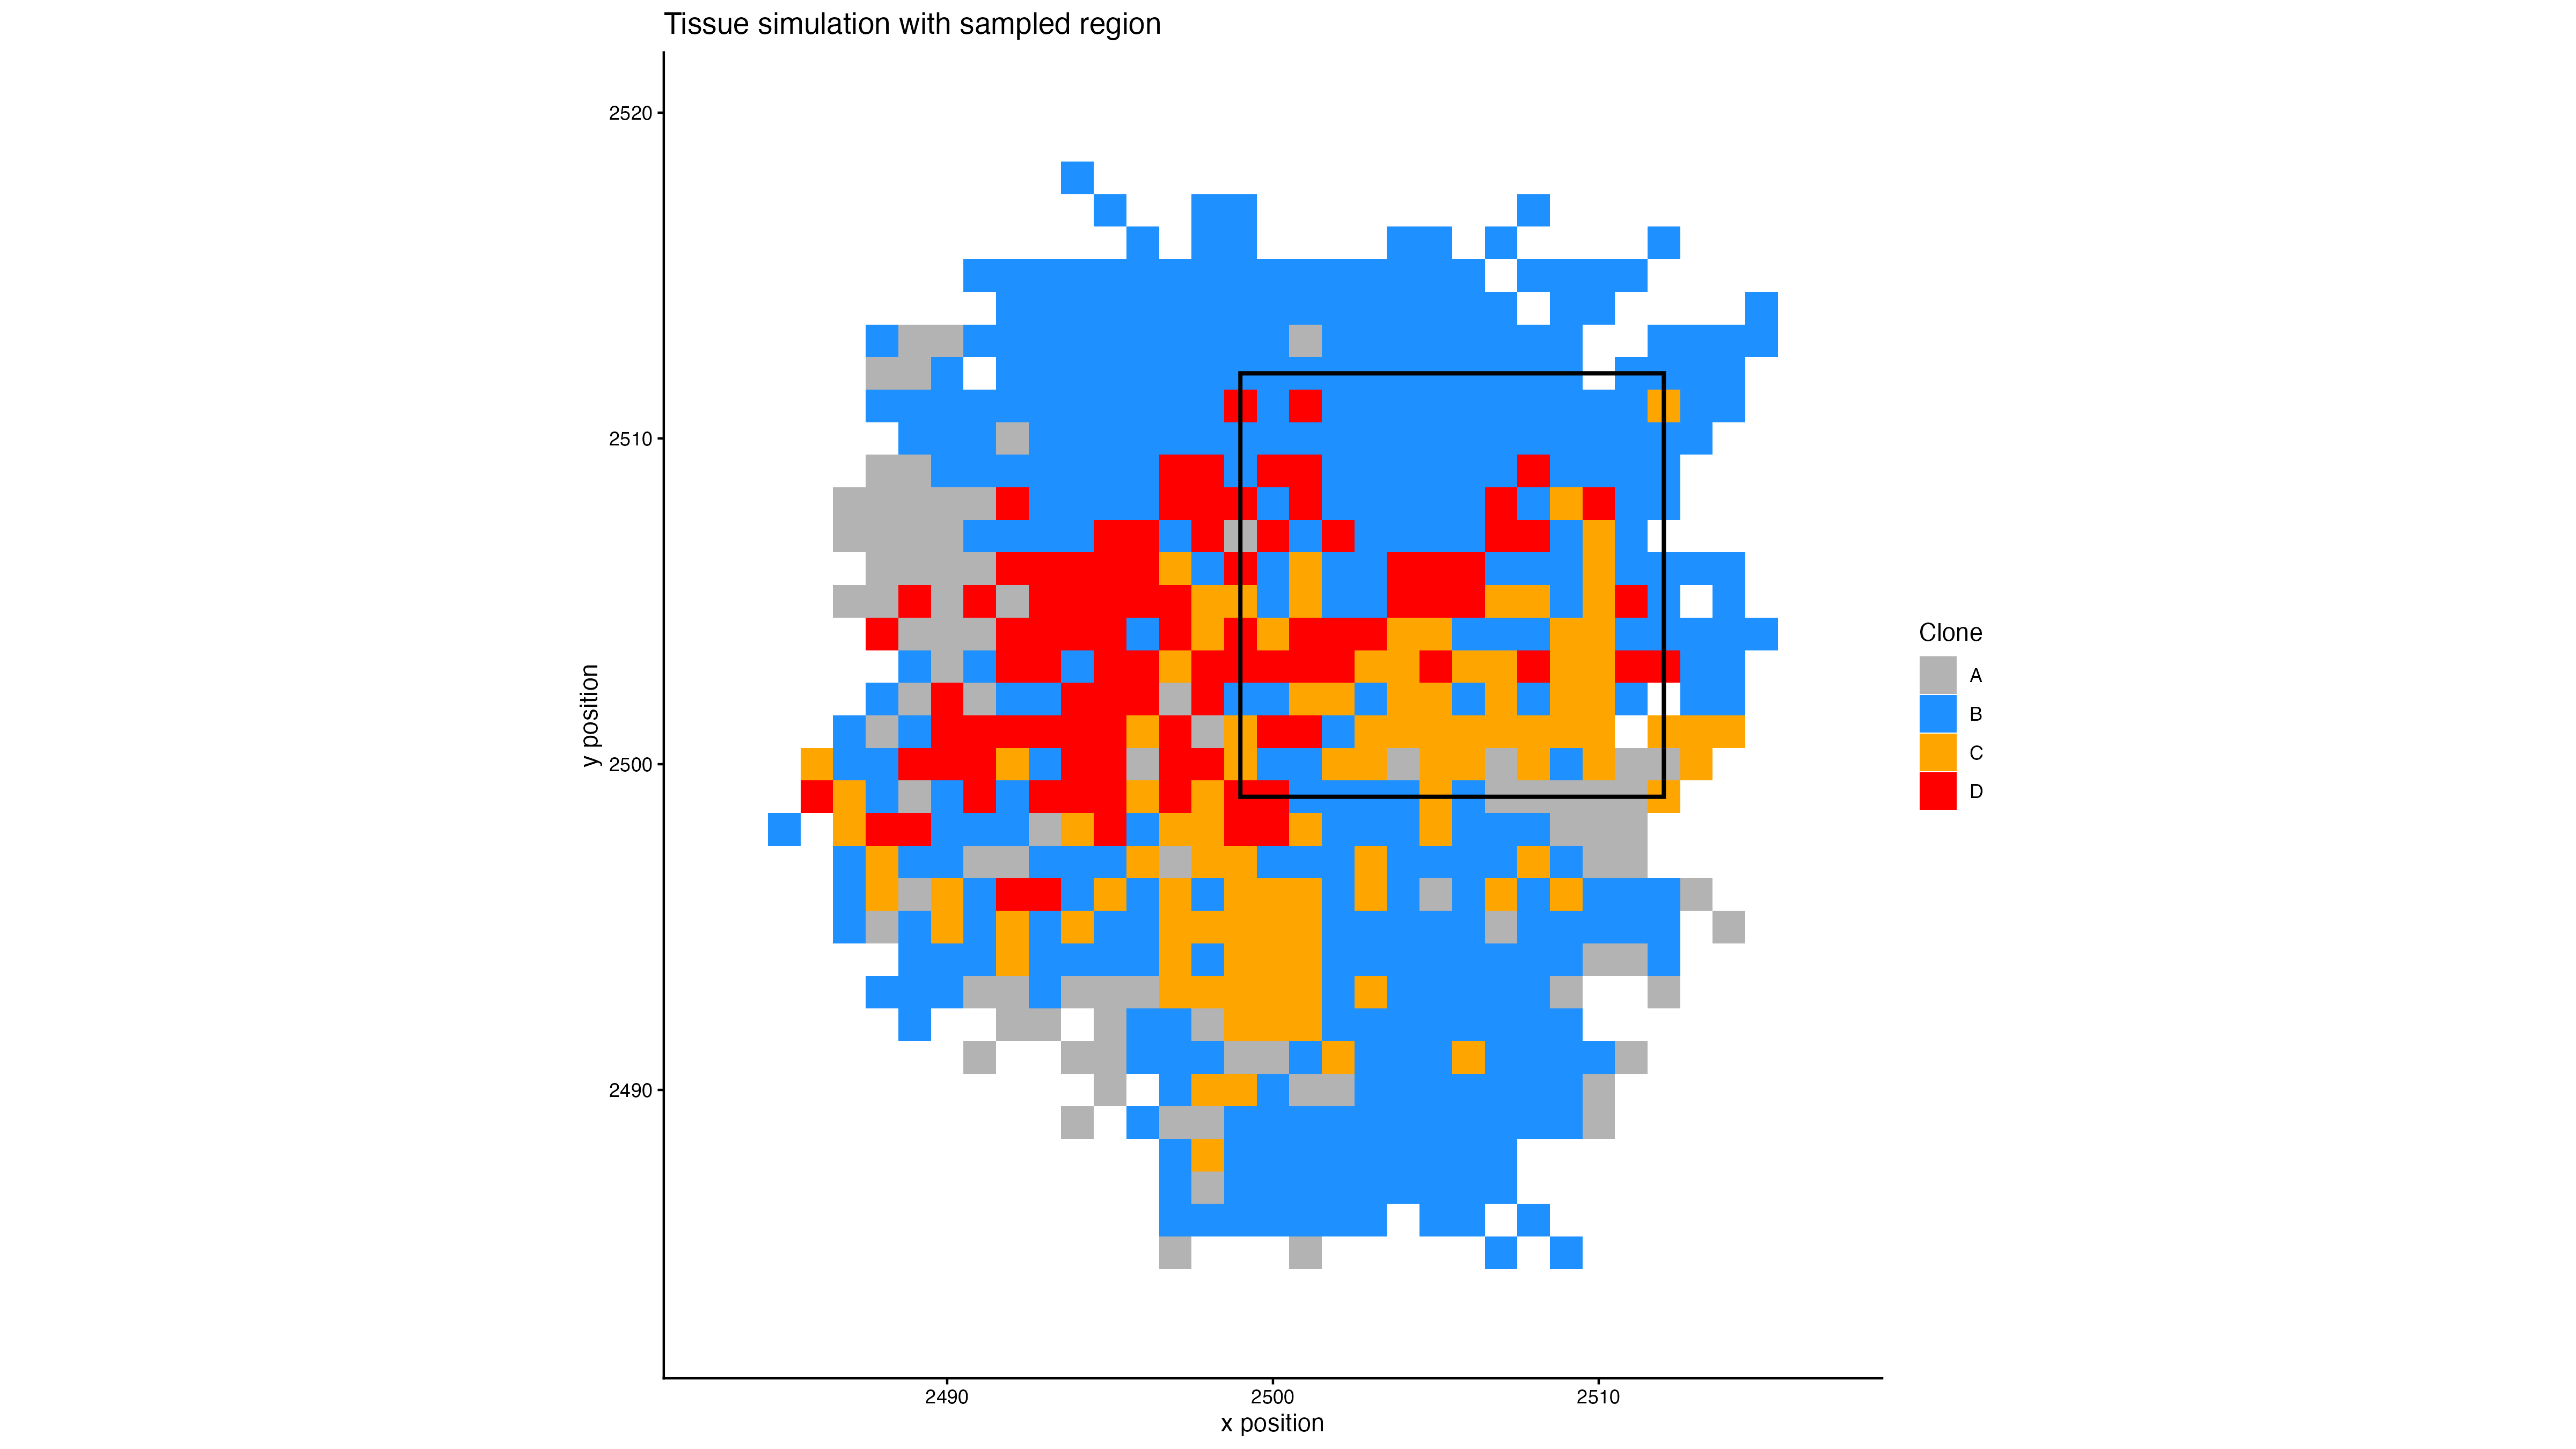
\includegraphics[width=0.8\linewidth]{immagini/figures 4 DLP/Tissue_Sampled_Plot.png}
    \captionsetup{font=footnotesize}
    \caption{The simulated four-clone tumour, each colour a clone; the black square
    marks the localized biopsy (DLP$^+$), a contiguous patch of tissue that over- and
    under-represents clones and so distorts the abundance signal.}
    \label{fig:c4d-sampled}
\end{figure}

\begin{figure}[H]
    \centering
    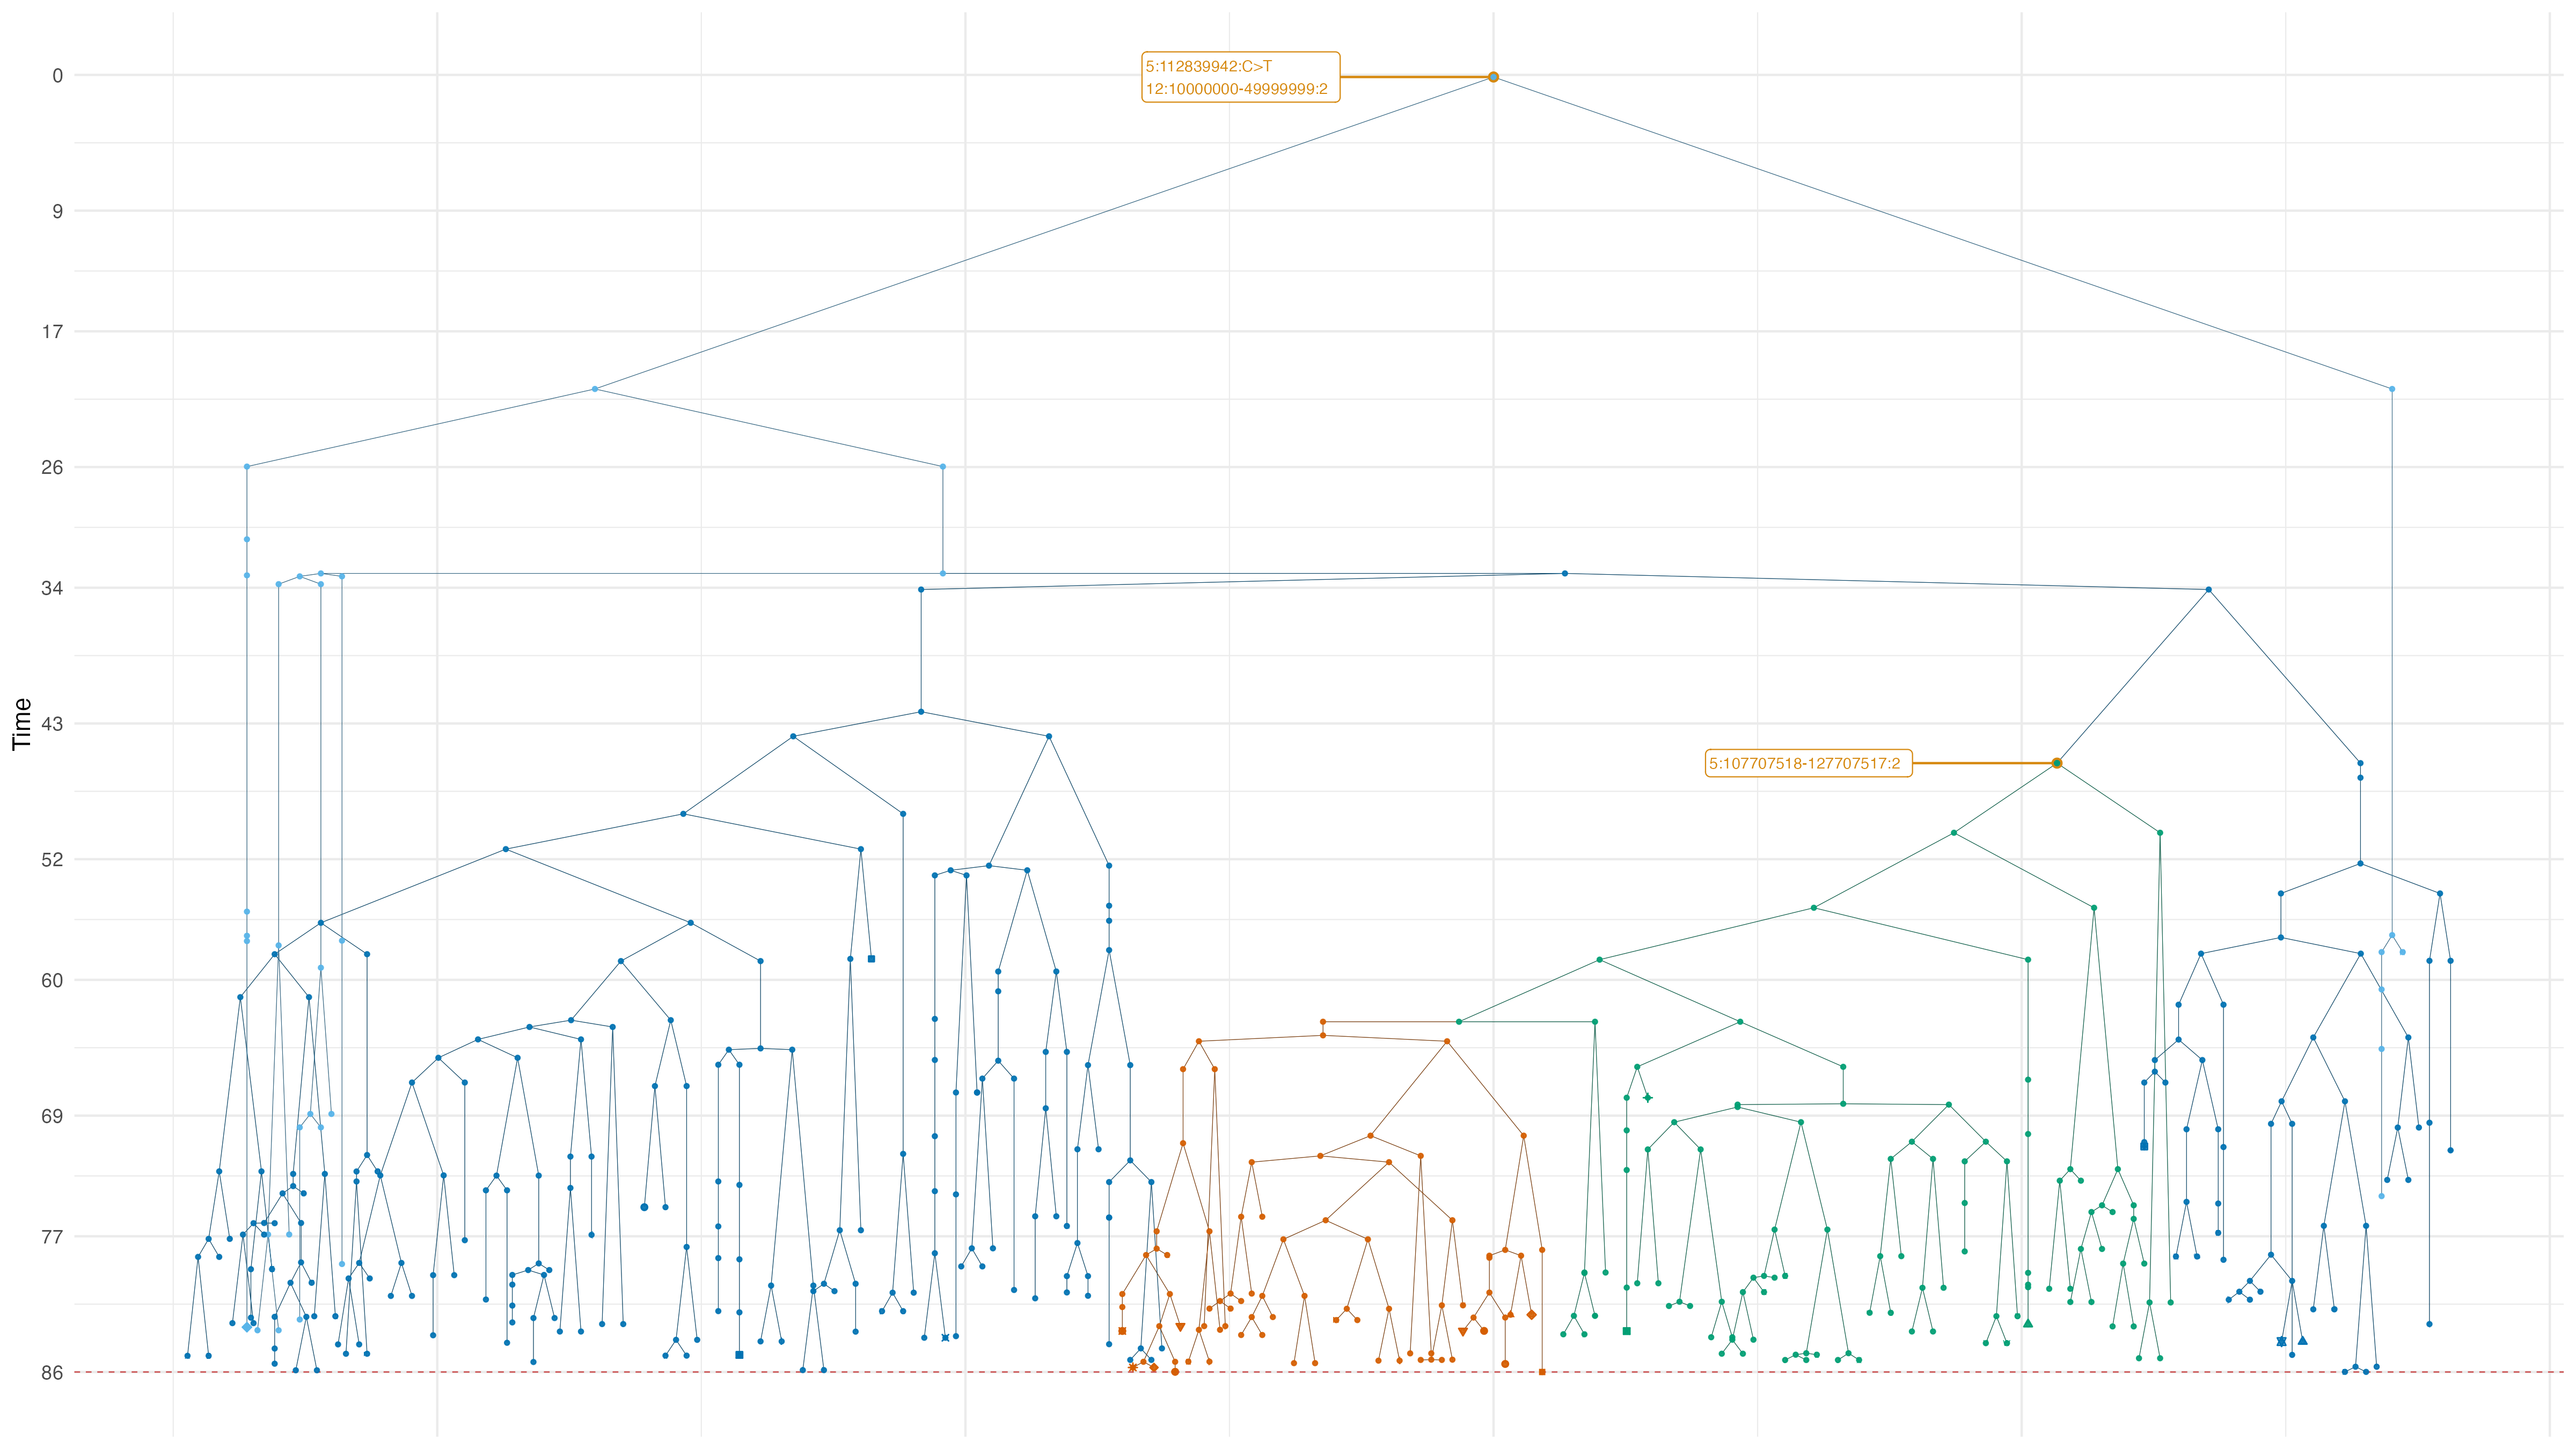
\includegraphics[width=0.8\linewidth]{immagini/figures 4 DLP/Forest_Mutations_Plot.png}
    \captionsetup{font=footnotesize}
    \caption{Mutation phylogeny reconstructed from the biopsy sample.}
    \label{fig:c4d-forest}
\end{figure}

\begin{figure}[H]
    \centering
    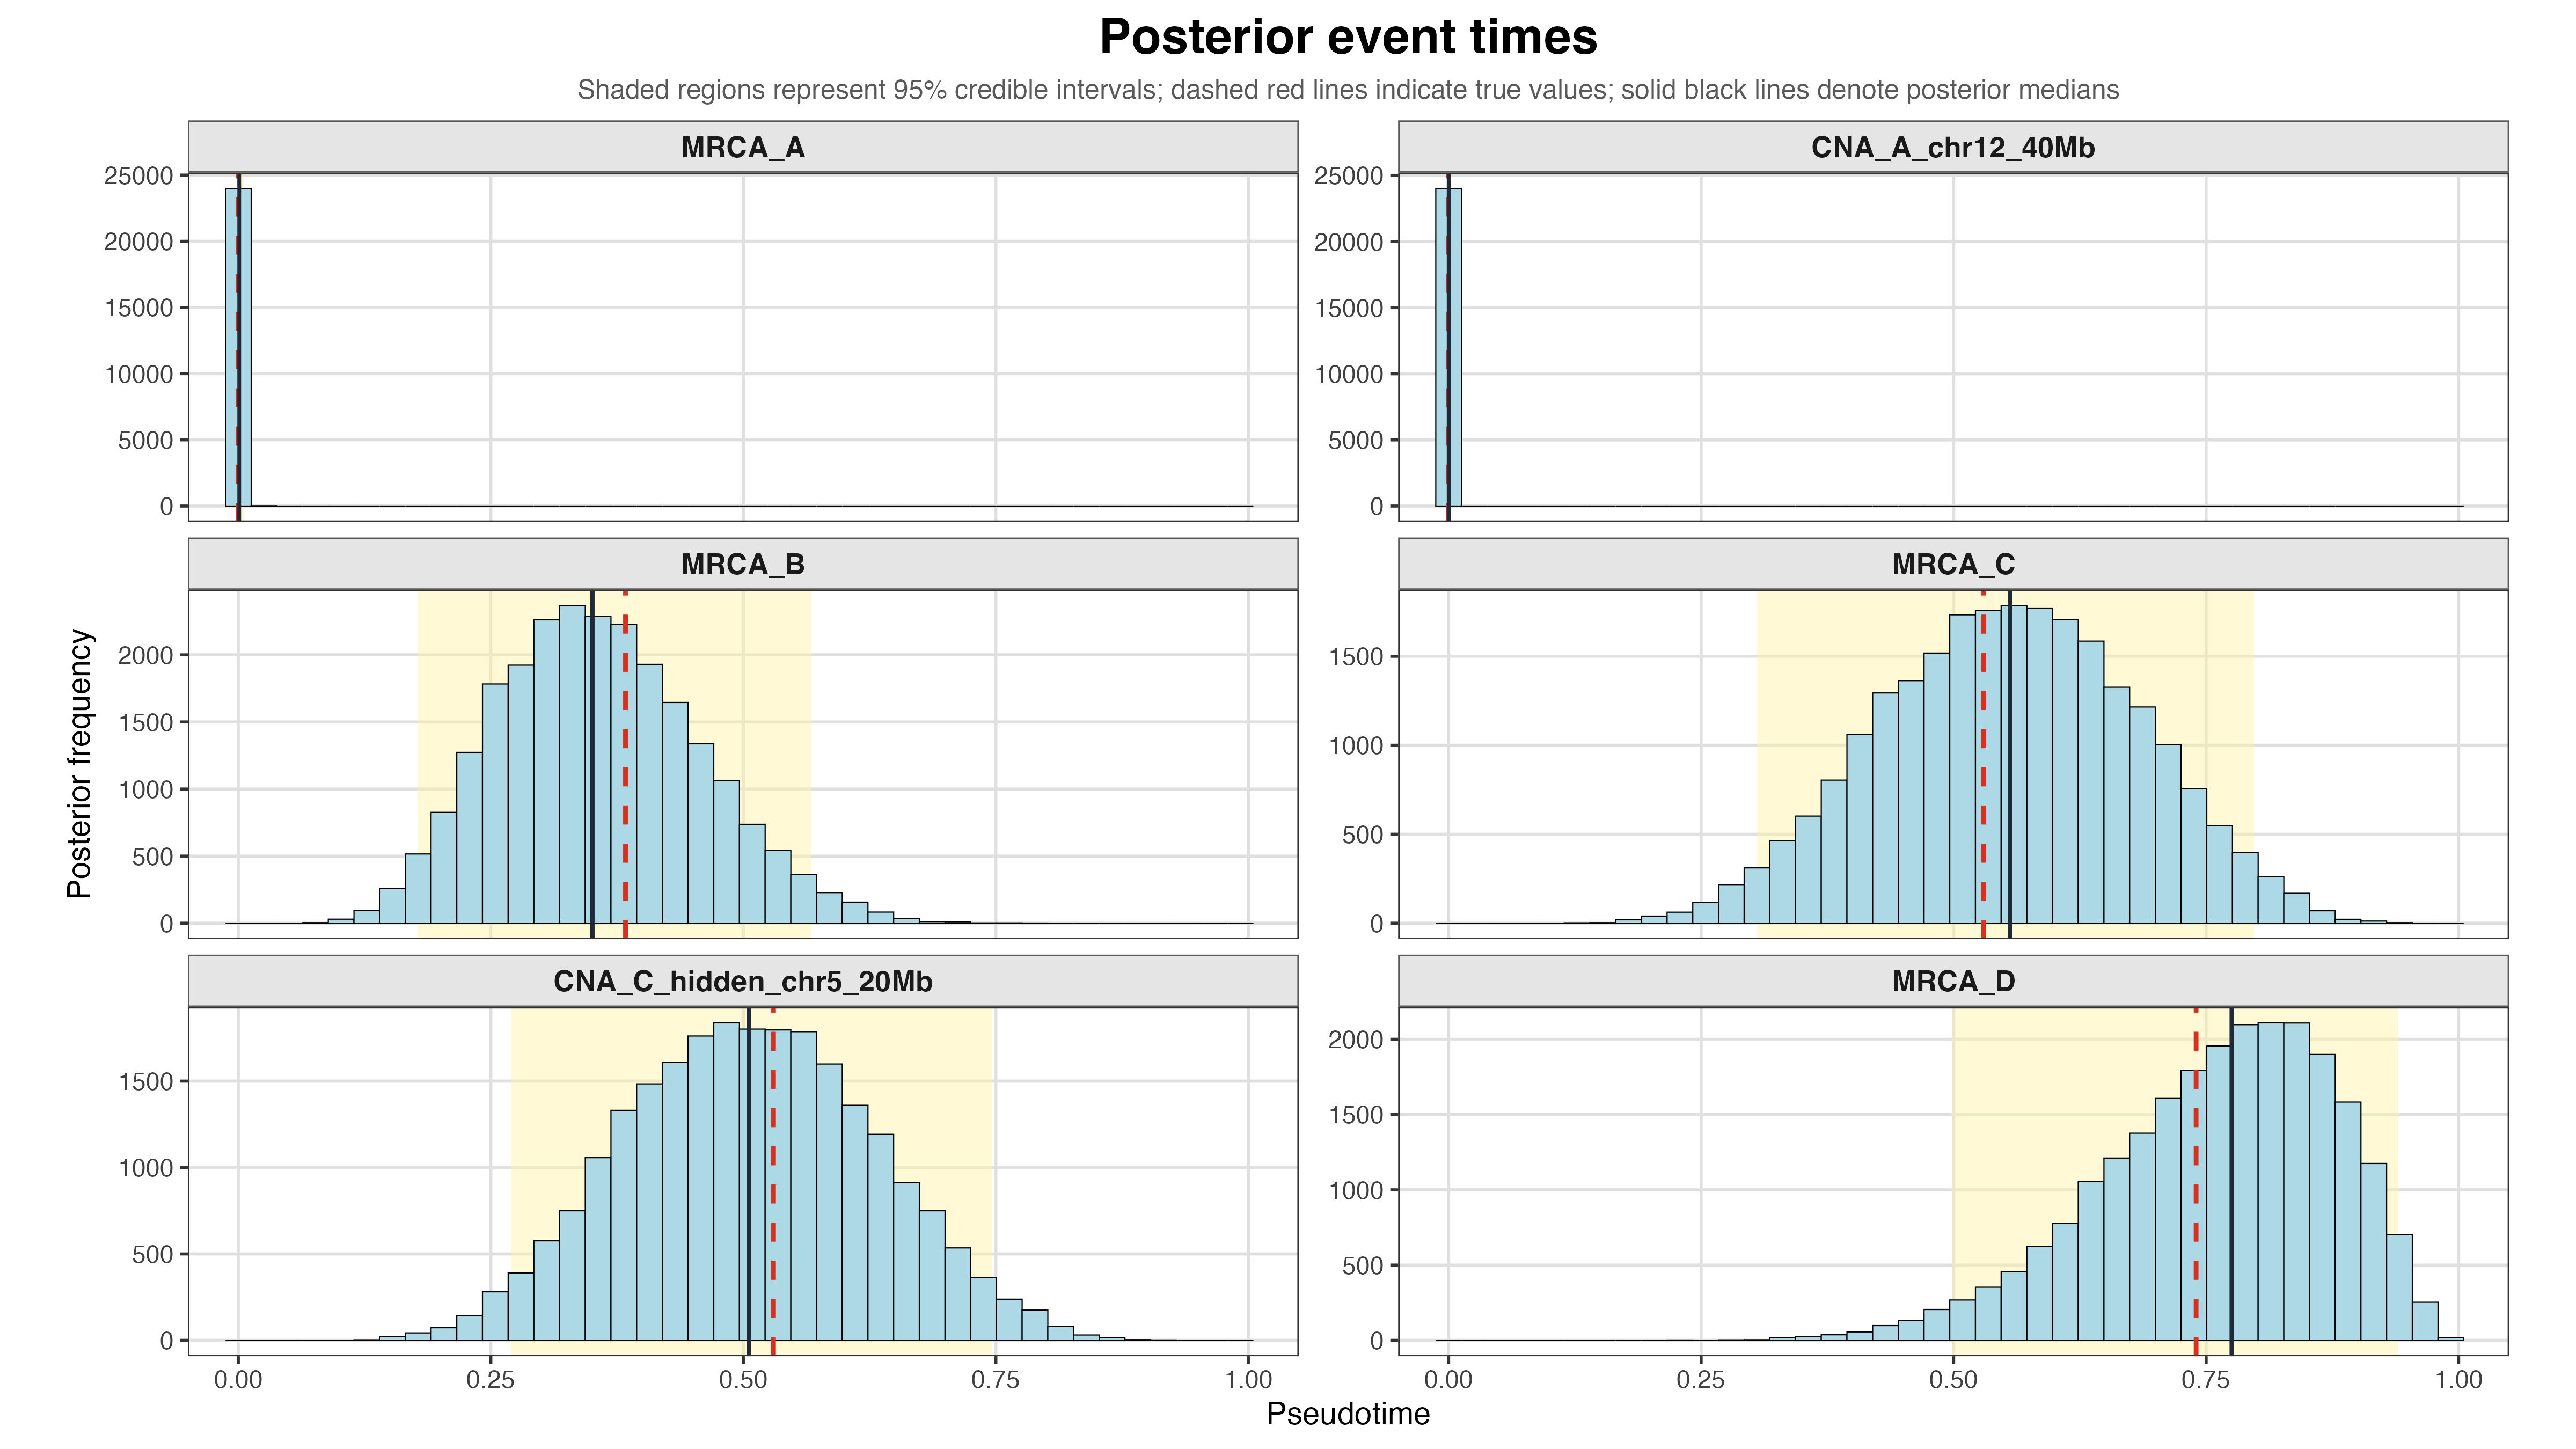
\includegraphics[width=0.8\linewidth]{immagini/figures 4 DLP/Posterior_Event_Times.png}
    \captionsetup{font=footnotesize}
    \caption{Posterior event pseudotimes against the ground truth (dashed) for the
    four-clone scenario; only the two root-clone events, fixed at $t\approx0$, fall
    outside their interval.}
    \label{fig:c4d-times}
\end{figure}

\begin{figure}[H]
    \centering
    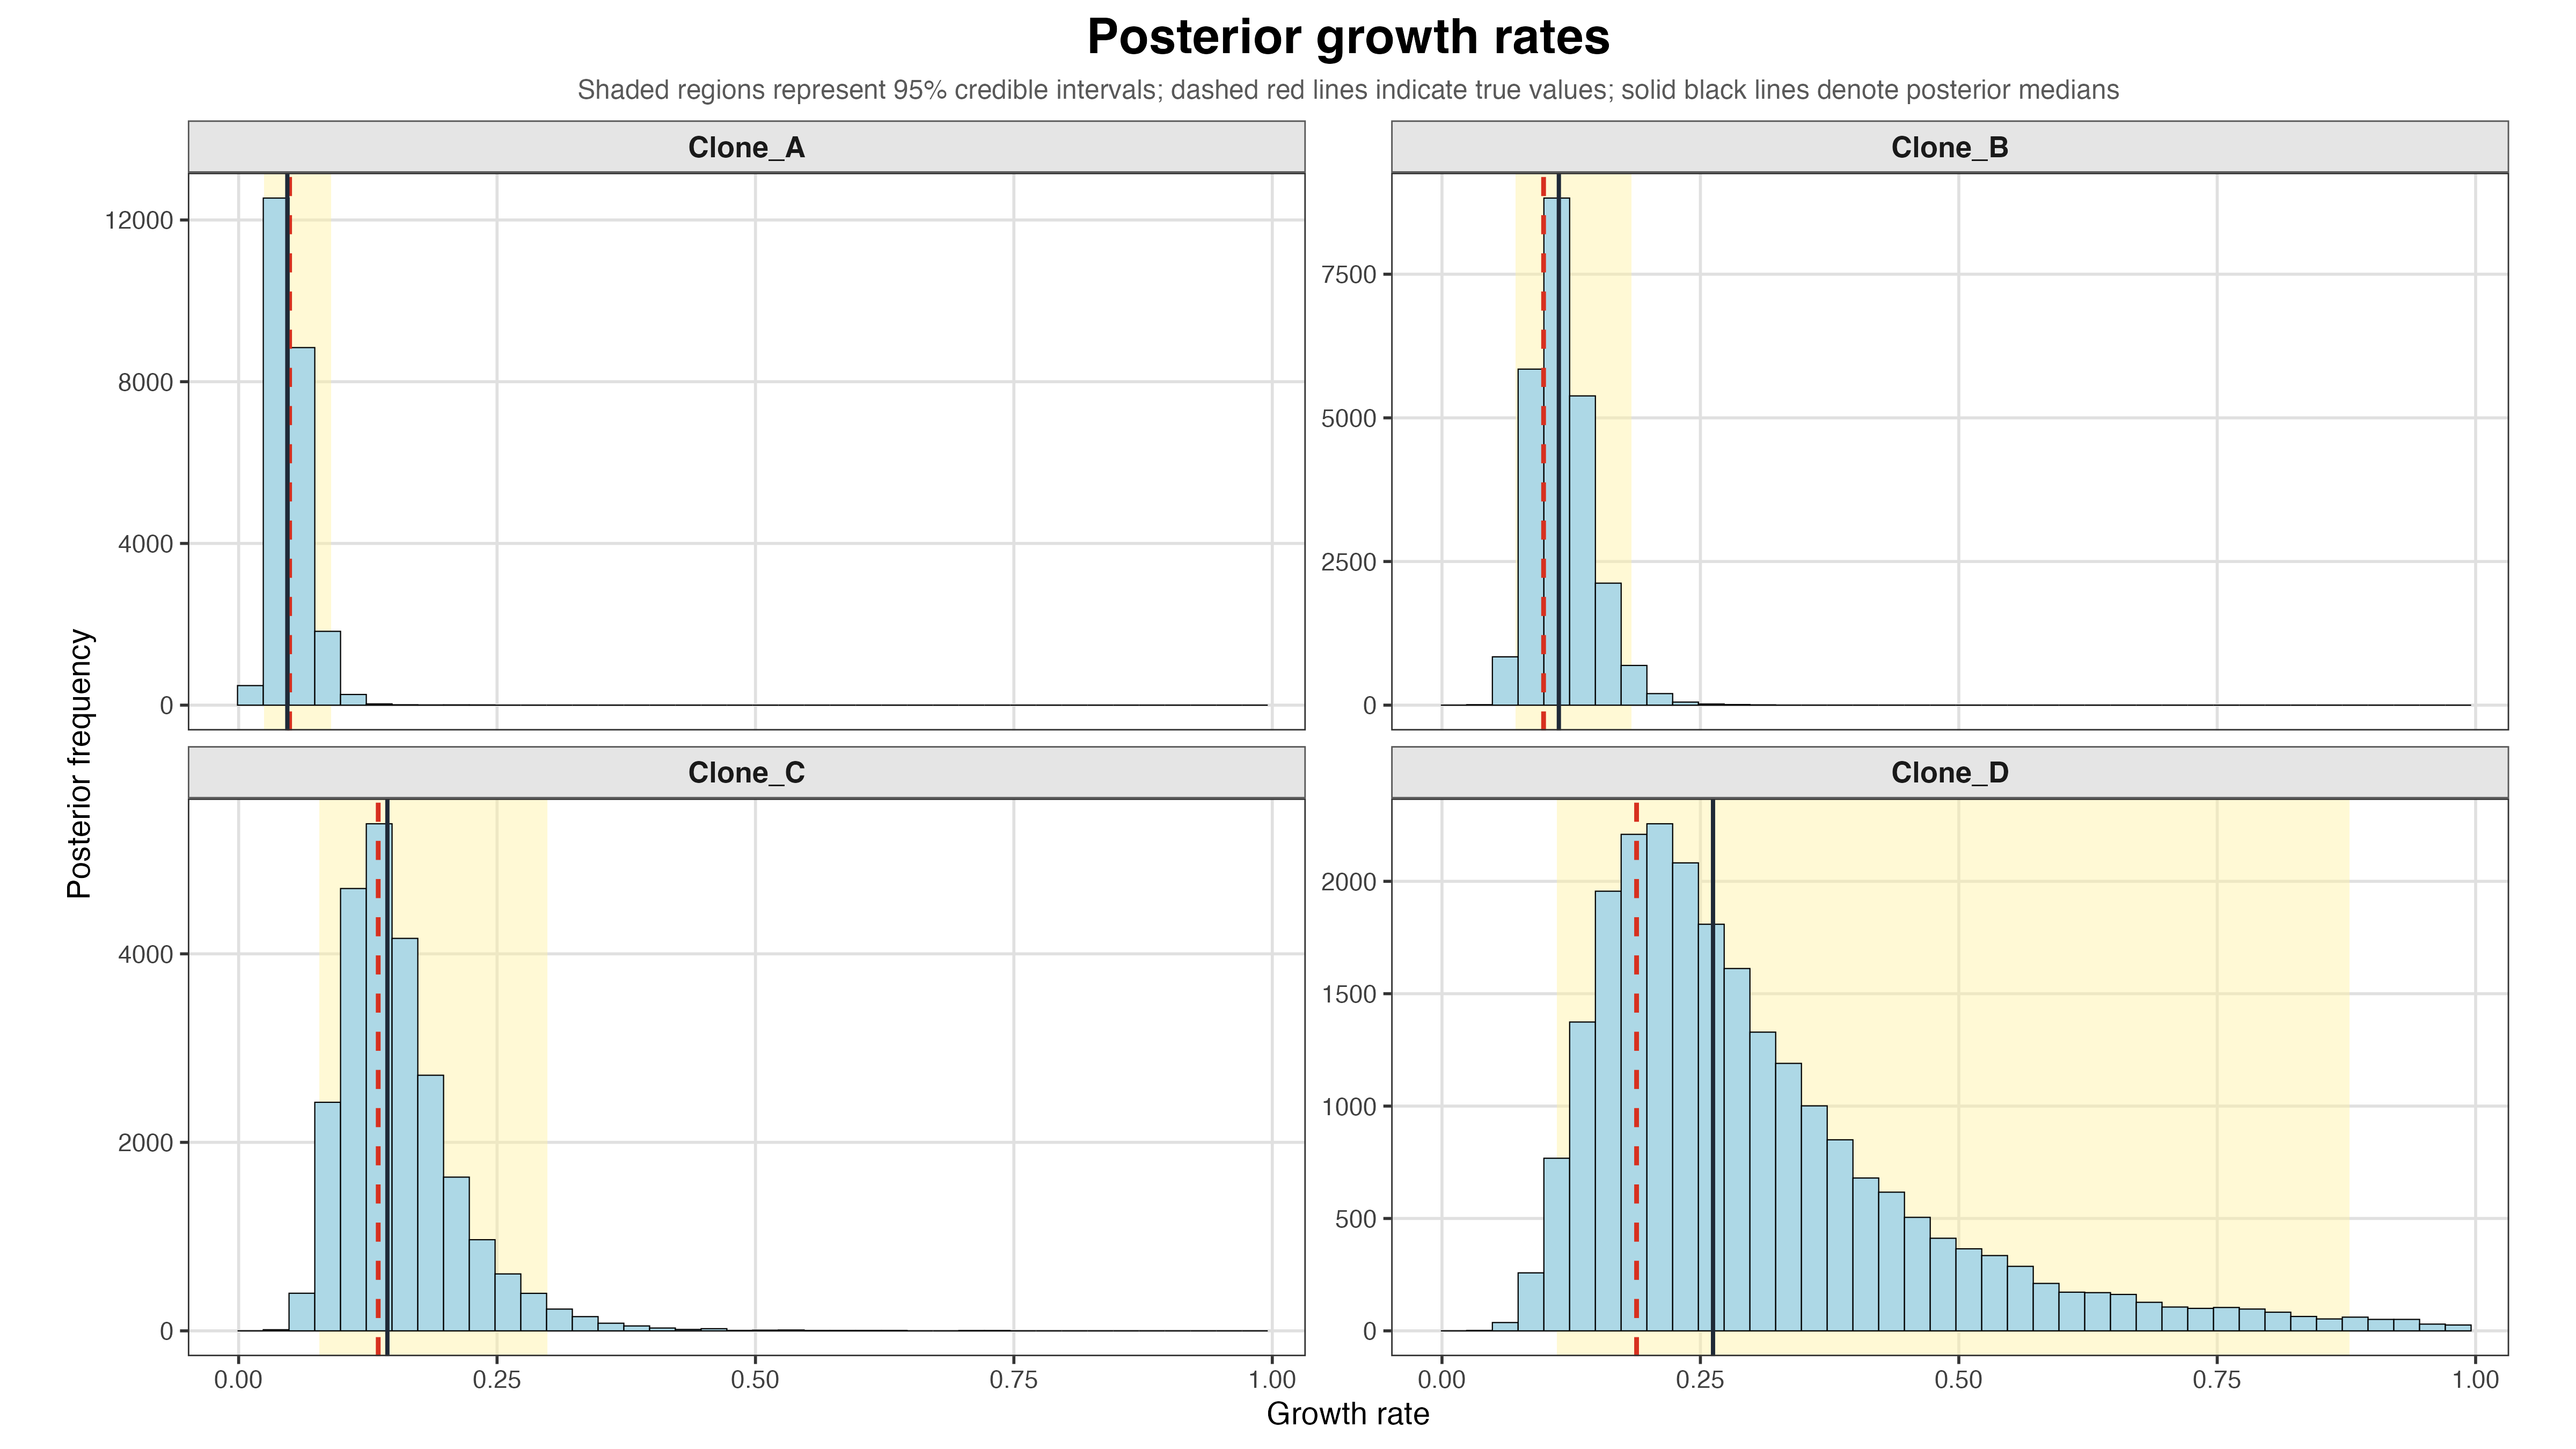
\includegraphics[width=0.8\linewidth]{immagini/figures 4 DLP/Posterior_Growth_Rates.png}
    \captionsetup{font=footnotesize}
    \caption{Posterior clone growth rates for the four-clone scenario under
    localized biopsy sampling.}
    \label{fig:c4d-growth}
\end{figure}

The mutation counts are intrinsic to each branch rather than to how the tissue is
sampled, so the biopsy distortion does not reach them. The posterior-predictive check
is satisfied on every one of the eight equations (Figure~\ref{fig:c4d-mut}): the
abundance distortion is absorbed by the model without leaking into the mutation
likelihood.

\begin{figure}[H]
    \centering
    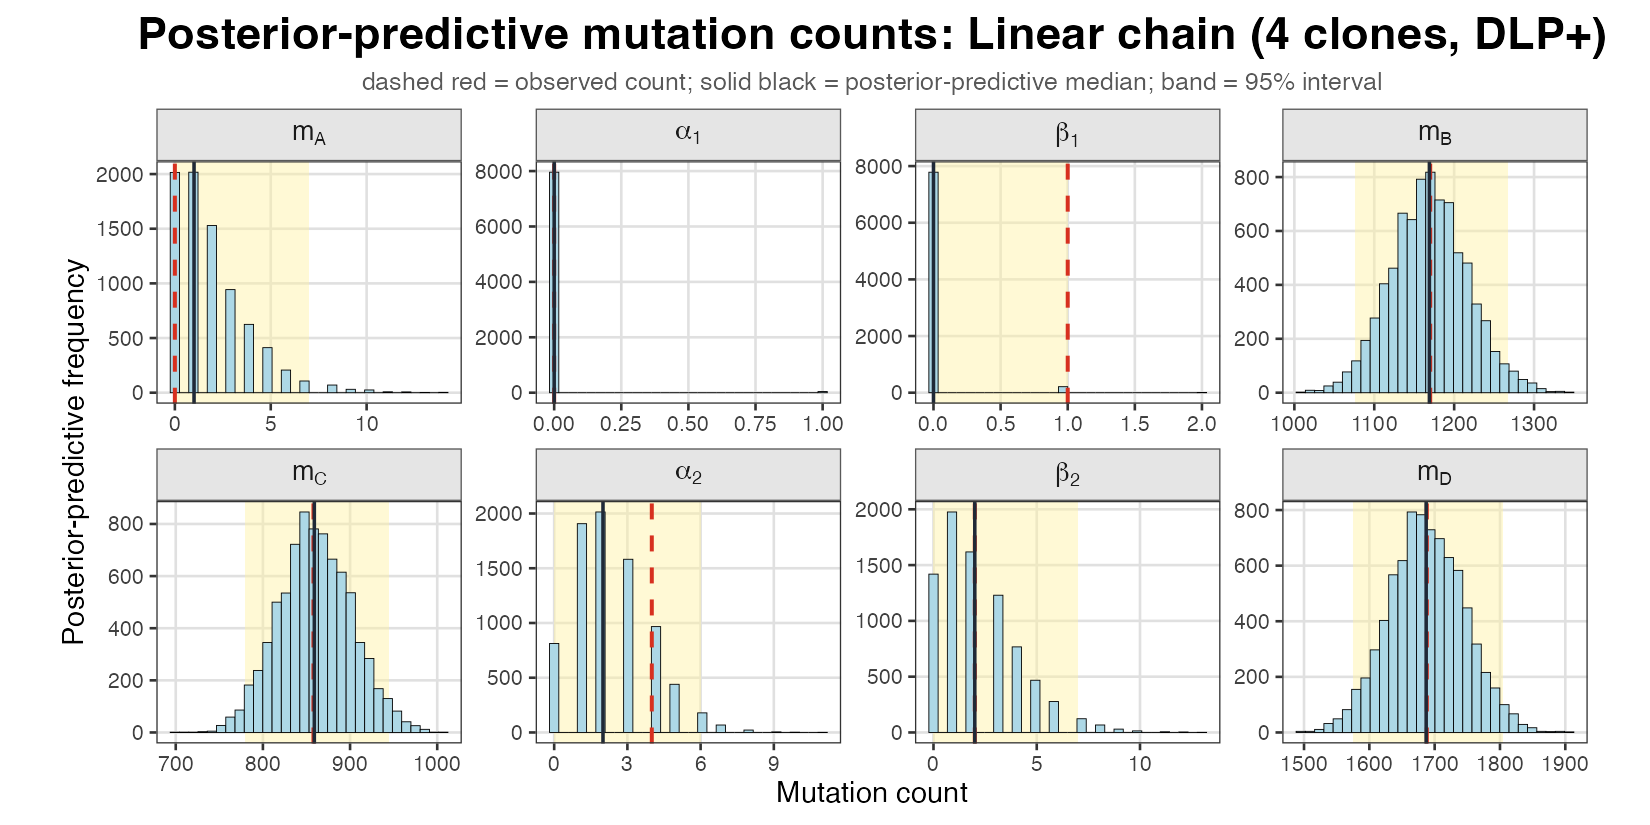
\includegraphics[width=\linewidth]{immagini/mut_dist_c4_dlp.png}
    \captionsetup{font=footnotesize}
    \caption{Posterior-predictive distribution of the mutation counts for the
    four-clone scenario. Each panel is one mutation equation; the dashed red line is
    the observed count, the solid line the predictive median, and the band the $95\%$
    predictive interval. All eight observed counts fall inside their intervals.}
    \label{fig:c4d-mut}
\end{figure}

Taken together, the four-clone scenario is a clean pass: despite the distorting
biopsy, the event times, the growth rates and the mutation counts are all recovered
within their credible intervals (Table~\ref{tab:sim-bias}). The gentlest ProCESS test
poses no real difficulty for the model.


\section{ProCESS: a branching six-clone tumour}
\begin{tcolorbox}[
  colback=white, colframe=procblue, boxrule=0.5pt, arc=2pt,
  before skip=2pt, after skip=4pt,
  top=0pt, bottom=3pt, left=4pt, right=4pt,
  boxsep=1pt,
  toptitle=2pt, bottomtitle=2pt,
  coltitle=white, colbacktitle=procblue, fonttitle=\bfseries\large,
  title={Branching tree (6 clones) \hfill \normalfont\normalsize Nnodes=6 \ \textbar\ Nevents=9 \ \textbar\ Nequations=12}
]
\begin{tcolorbox}[colback=white, colframe=procblue!55, boxrule=0.4pt, arc=1pt,
  before skip=0pt, after skip=4pt, left=3pt, right=3pt, top=3pt, bottom=3pt]
\textbf{Topology}\quad (branching, 6 sampled, 0 hidden)\\[4pt]
\cnode{Clone\_A} $\longrightarrow$ \cnode{Clone\_B} $\longrightarrow$ \cnode{Clone\_C} $\longrightarrow$ \cnode{Clone\_E}\\[2pt]
\phantom{\cnode{Clone\_A} $\longrightarrow$ \cnode{Clone\_B} }$\searrow$\ \cnode{Clone\_D} $\longrightarrow$ \cnode{Clone\_F}
\end{tcolorbox}
\vspace{2pt}
\begin{tabular}{@{}ll@{}}
\toprule
\textbf{Sampled}            & Clone\_A, Clone\_B, Clone\_C, Clone\_D, Clone\_E, Clone\_F \\
\textbf{Sampling}           & localized biopsy (DLP$^+$) \\
\textbf{Stan parents}       & (0, 1, 2, 2, 3, 4) \\
\textbf{number\_of\_events} & (2, 1, 2, 2, 1, 1) \\
\midrule
\textbf{CNAs}               & CNA\_A on Clone\_A -- chr12, 40\,Mb \\
                            & CNA\_C\_hidden in Clone\_C -- chr5, 20\,Mb \\
                            & CNA\_D\_hidden in Clone\_D -- chr18, 20\,Mb \\
\midrule
\textbf{Growth rates}       & $w_A{=}0.0493$\quad $w_B{=}0.0920$\quad $w_C{=}0.0946$ \\
                            & $w_D{=}0.0969$\quad $w_E{=}0.1879$\quad $w_F{=}0.1165$ \\
\textbf{Equal rates}        & none \\
\bottomrule
\end{tabular}
\end{tcolorbox}


The biopsy of the six-clone tumour returned $1369$ cells, dominated by the leaf clone
$E$ ($883$) and very sparse for $C$ (only $8$): the strongly skewed composition a
focal sample produces in practice ($107$, $267$, $8$, $37$, $883$, $67$ for clones
$A$--$F$). Sequencing is at $T_f\approx 141$ on the simulator's clock; the clones are
born at pseudotimes $t_B=0.29$, $t_C=0.60$, $t_D=0.72$, $t_E=0.74$, $t_F=0.77$ (real
times $\approx 41$, $85$, $101$, $104$ and $108$), and copy-number events sit on $A$,
$C$ and $D$. Growth rates and CNAs are those of the card above; recovery is
summarised in Table~\ref{tab:sim-bias}.

The six-clone branching tree, carrying three copy-number events, is the harder
problem, and it is here that the identifiability limit anticipated by the ideal-DGP
analysis becomes visible. The pseudotimes are recovered with a mean absolute error of
$0.056$, larger than on the four-clone chain, with the root events again among those
left uncovered (Figure~\ref{fig:c6d-times}). The growth rates carry a larger relative
error, around $22\%$ (Figure~\ref{fig:c6d-growth}): exactly the single-snapshot floor
predicted on a deeper tree. The intervals still cover the truth for all six clones, so
rather than settling on a wrong value the model widens its uncertainty, as under the
ideal DGP.

\begin{figure}[H]
    \centering
    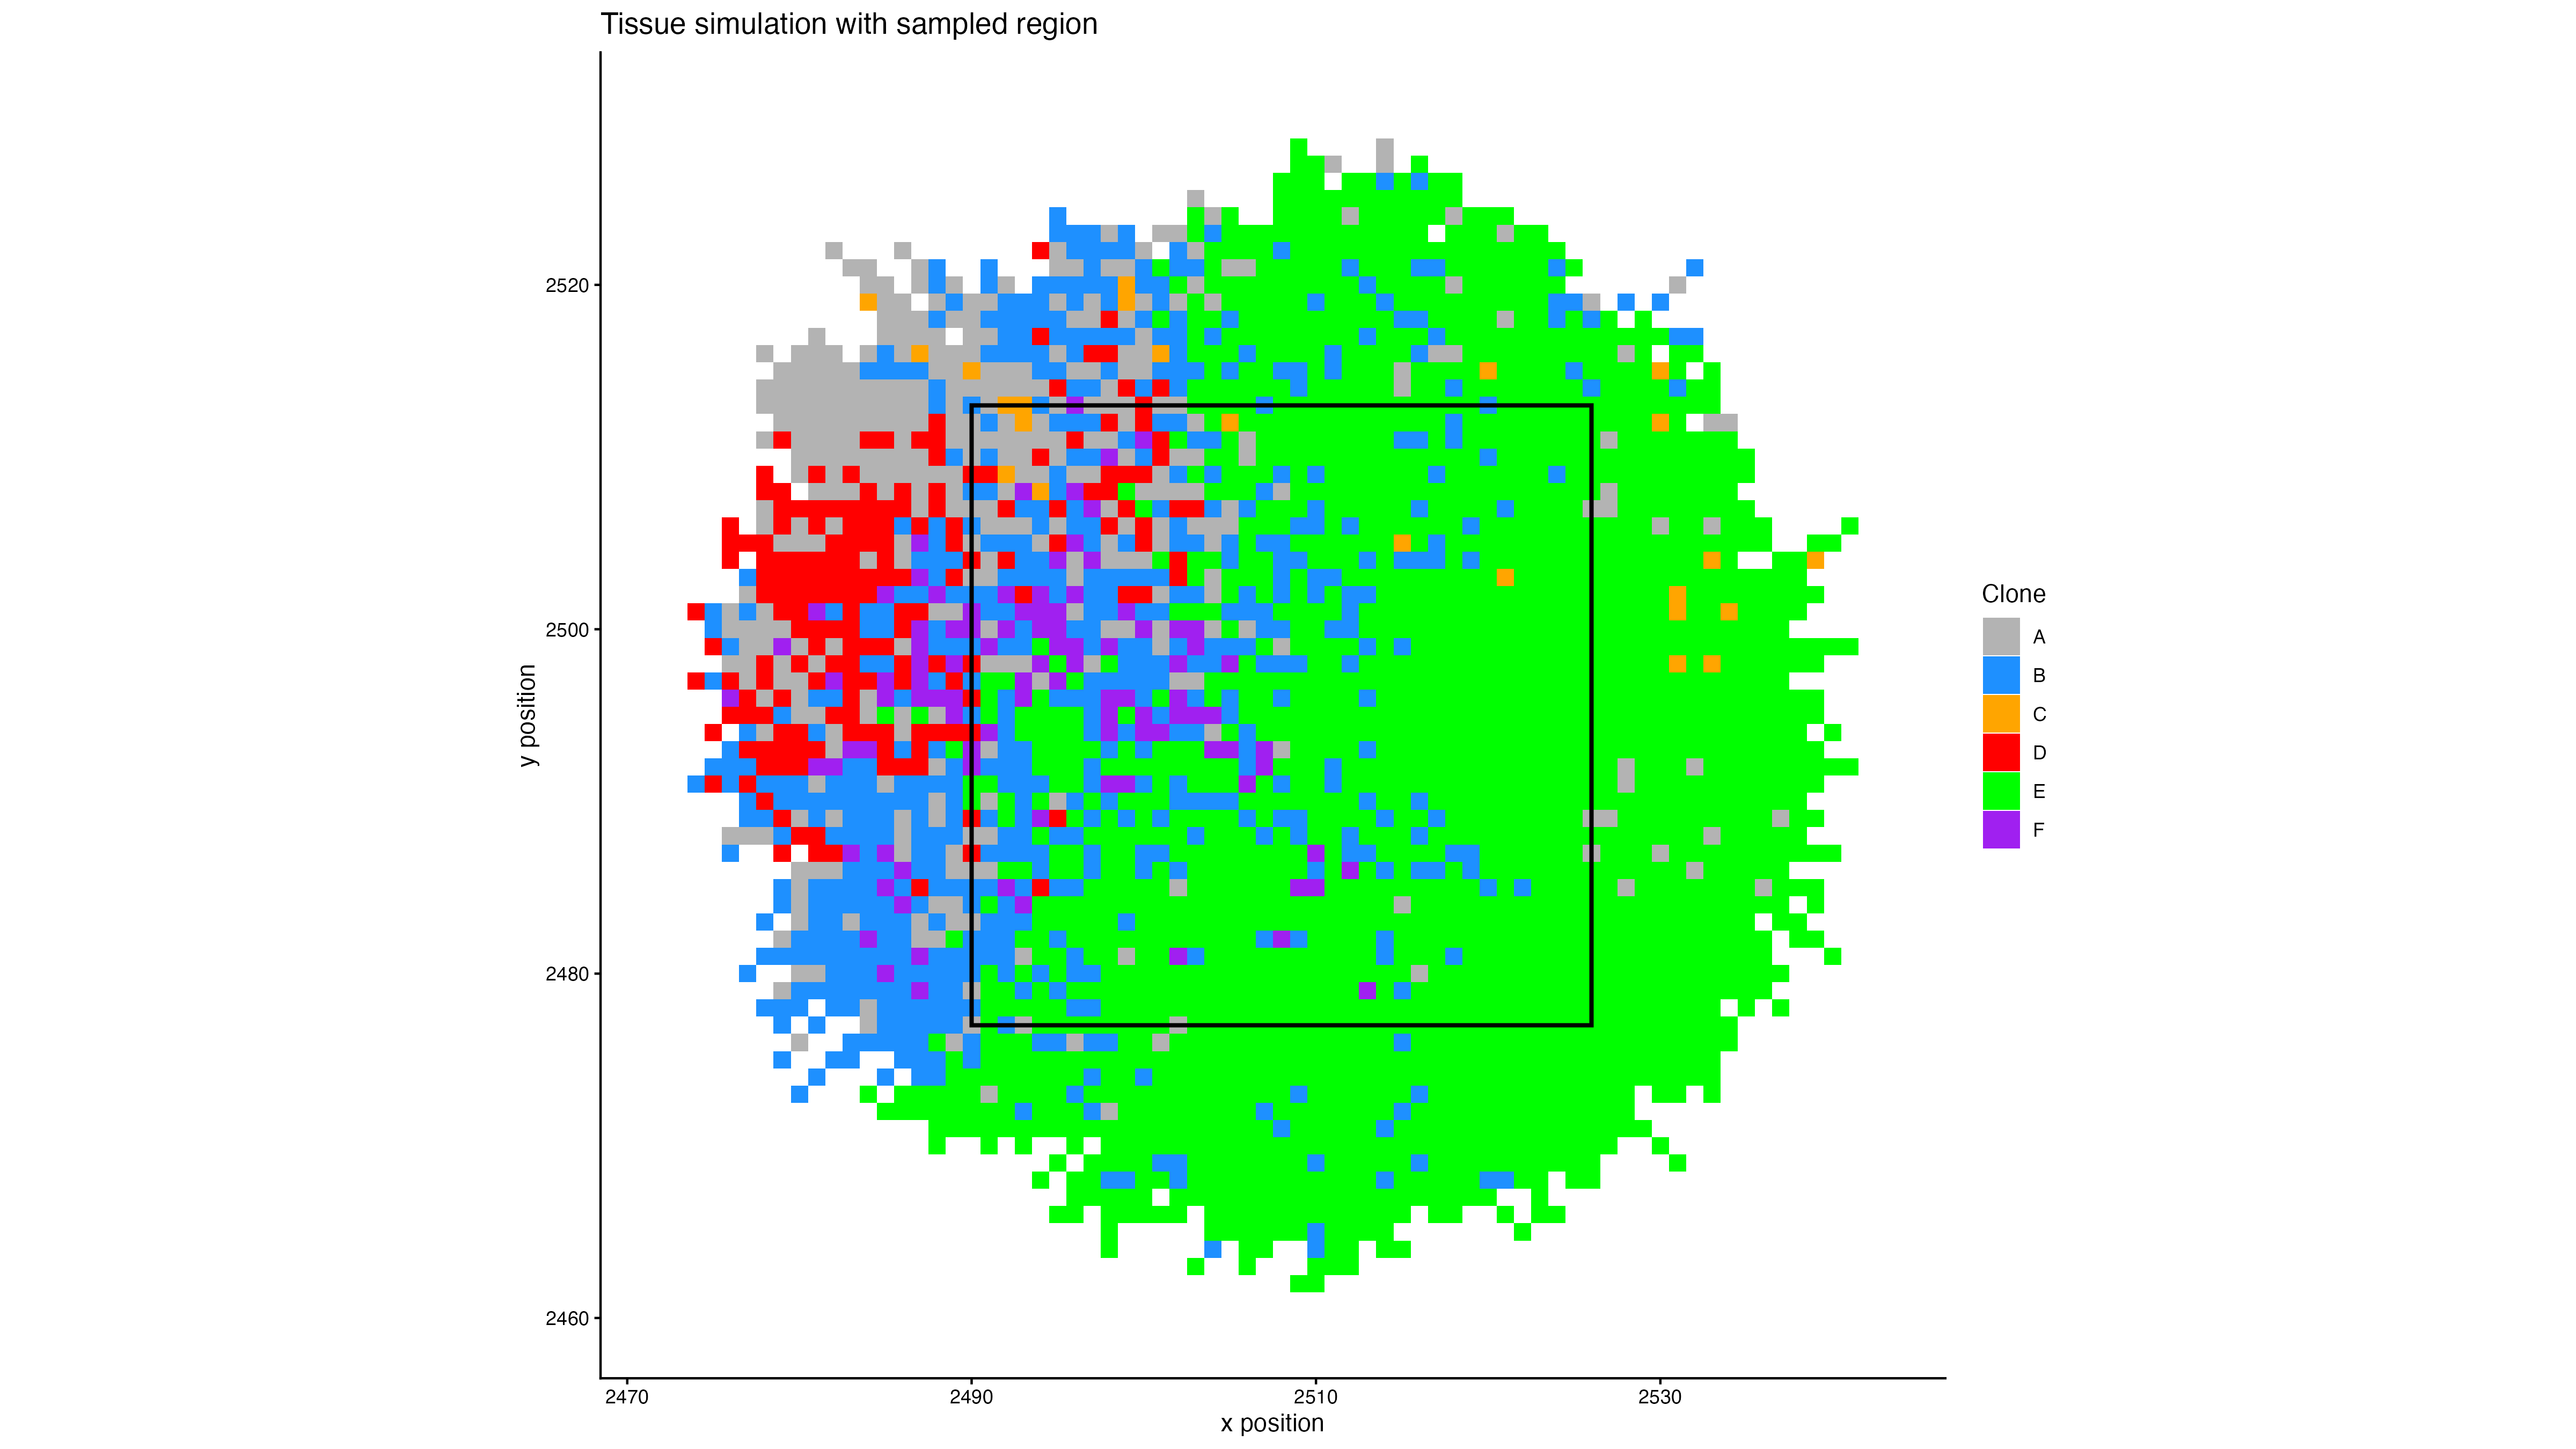
\includegraphics[width=0.8\linewidth]{immagini/figures 6 DLP/Tissue_Sampled_Plot.png}
    \captionsetup{font=footnotesize}
    \caption{The simulated six-clone branching tumour, each colour a clone; the black
    square marks the localized biopsy (DLP$^+$) used to sample it.}
    \label{fig:c6d-sampled}
\end{figure}

\begin{figure}[H]
    \centering
    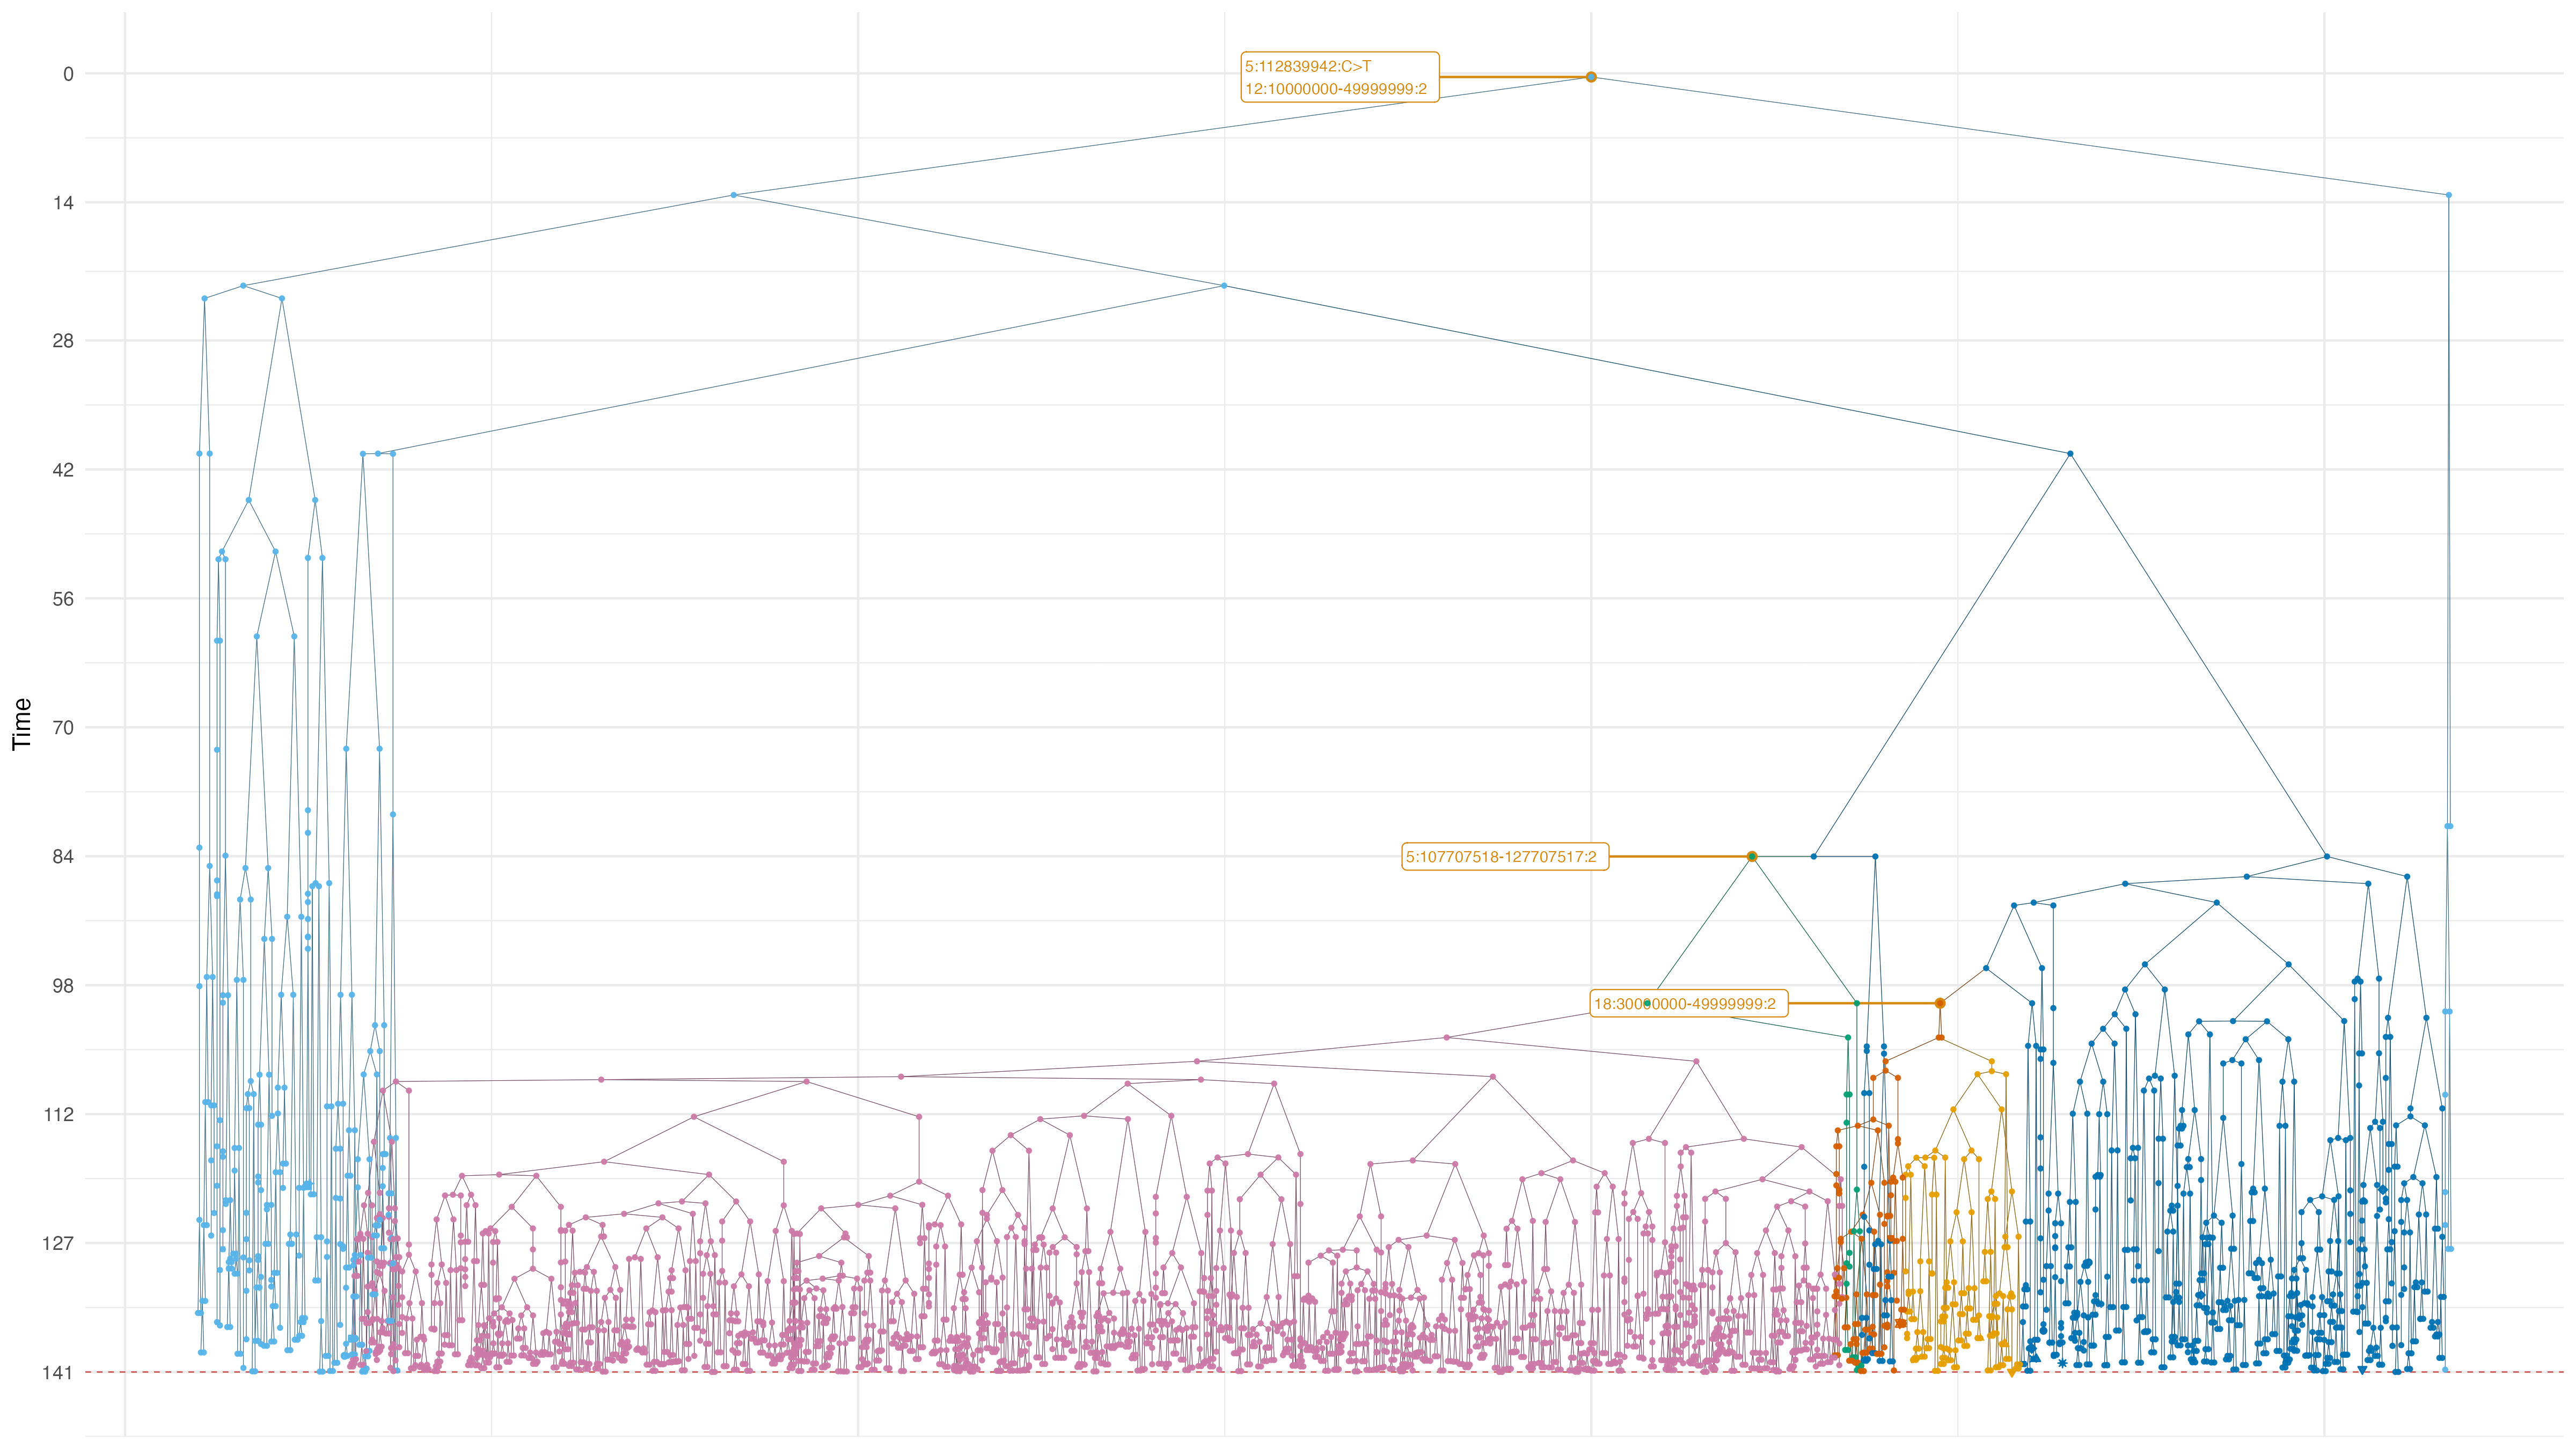
\includegraphics[width=0.8\linewidth]{immagini/figures 6 DLP/Forest_Mutations_Plot.png}
    \captionsetup{font=footnotesize}
    \caption{Mutation phylogeny reconstructed from the biopsy sample of the
    six-clone tumour.}
    \label{fig:c6d-forest}
\end{figure}

\begin{figure}[H]
    \centering
    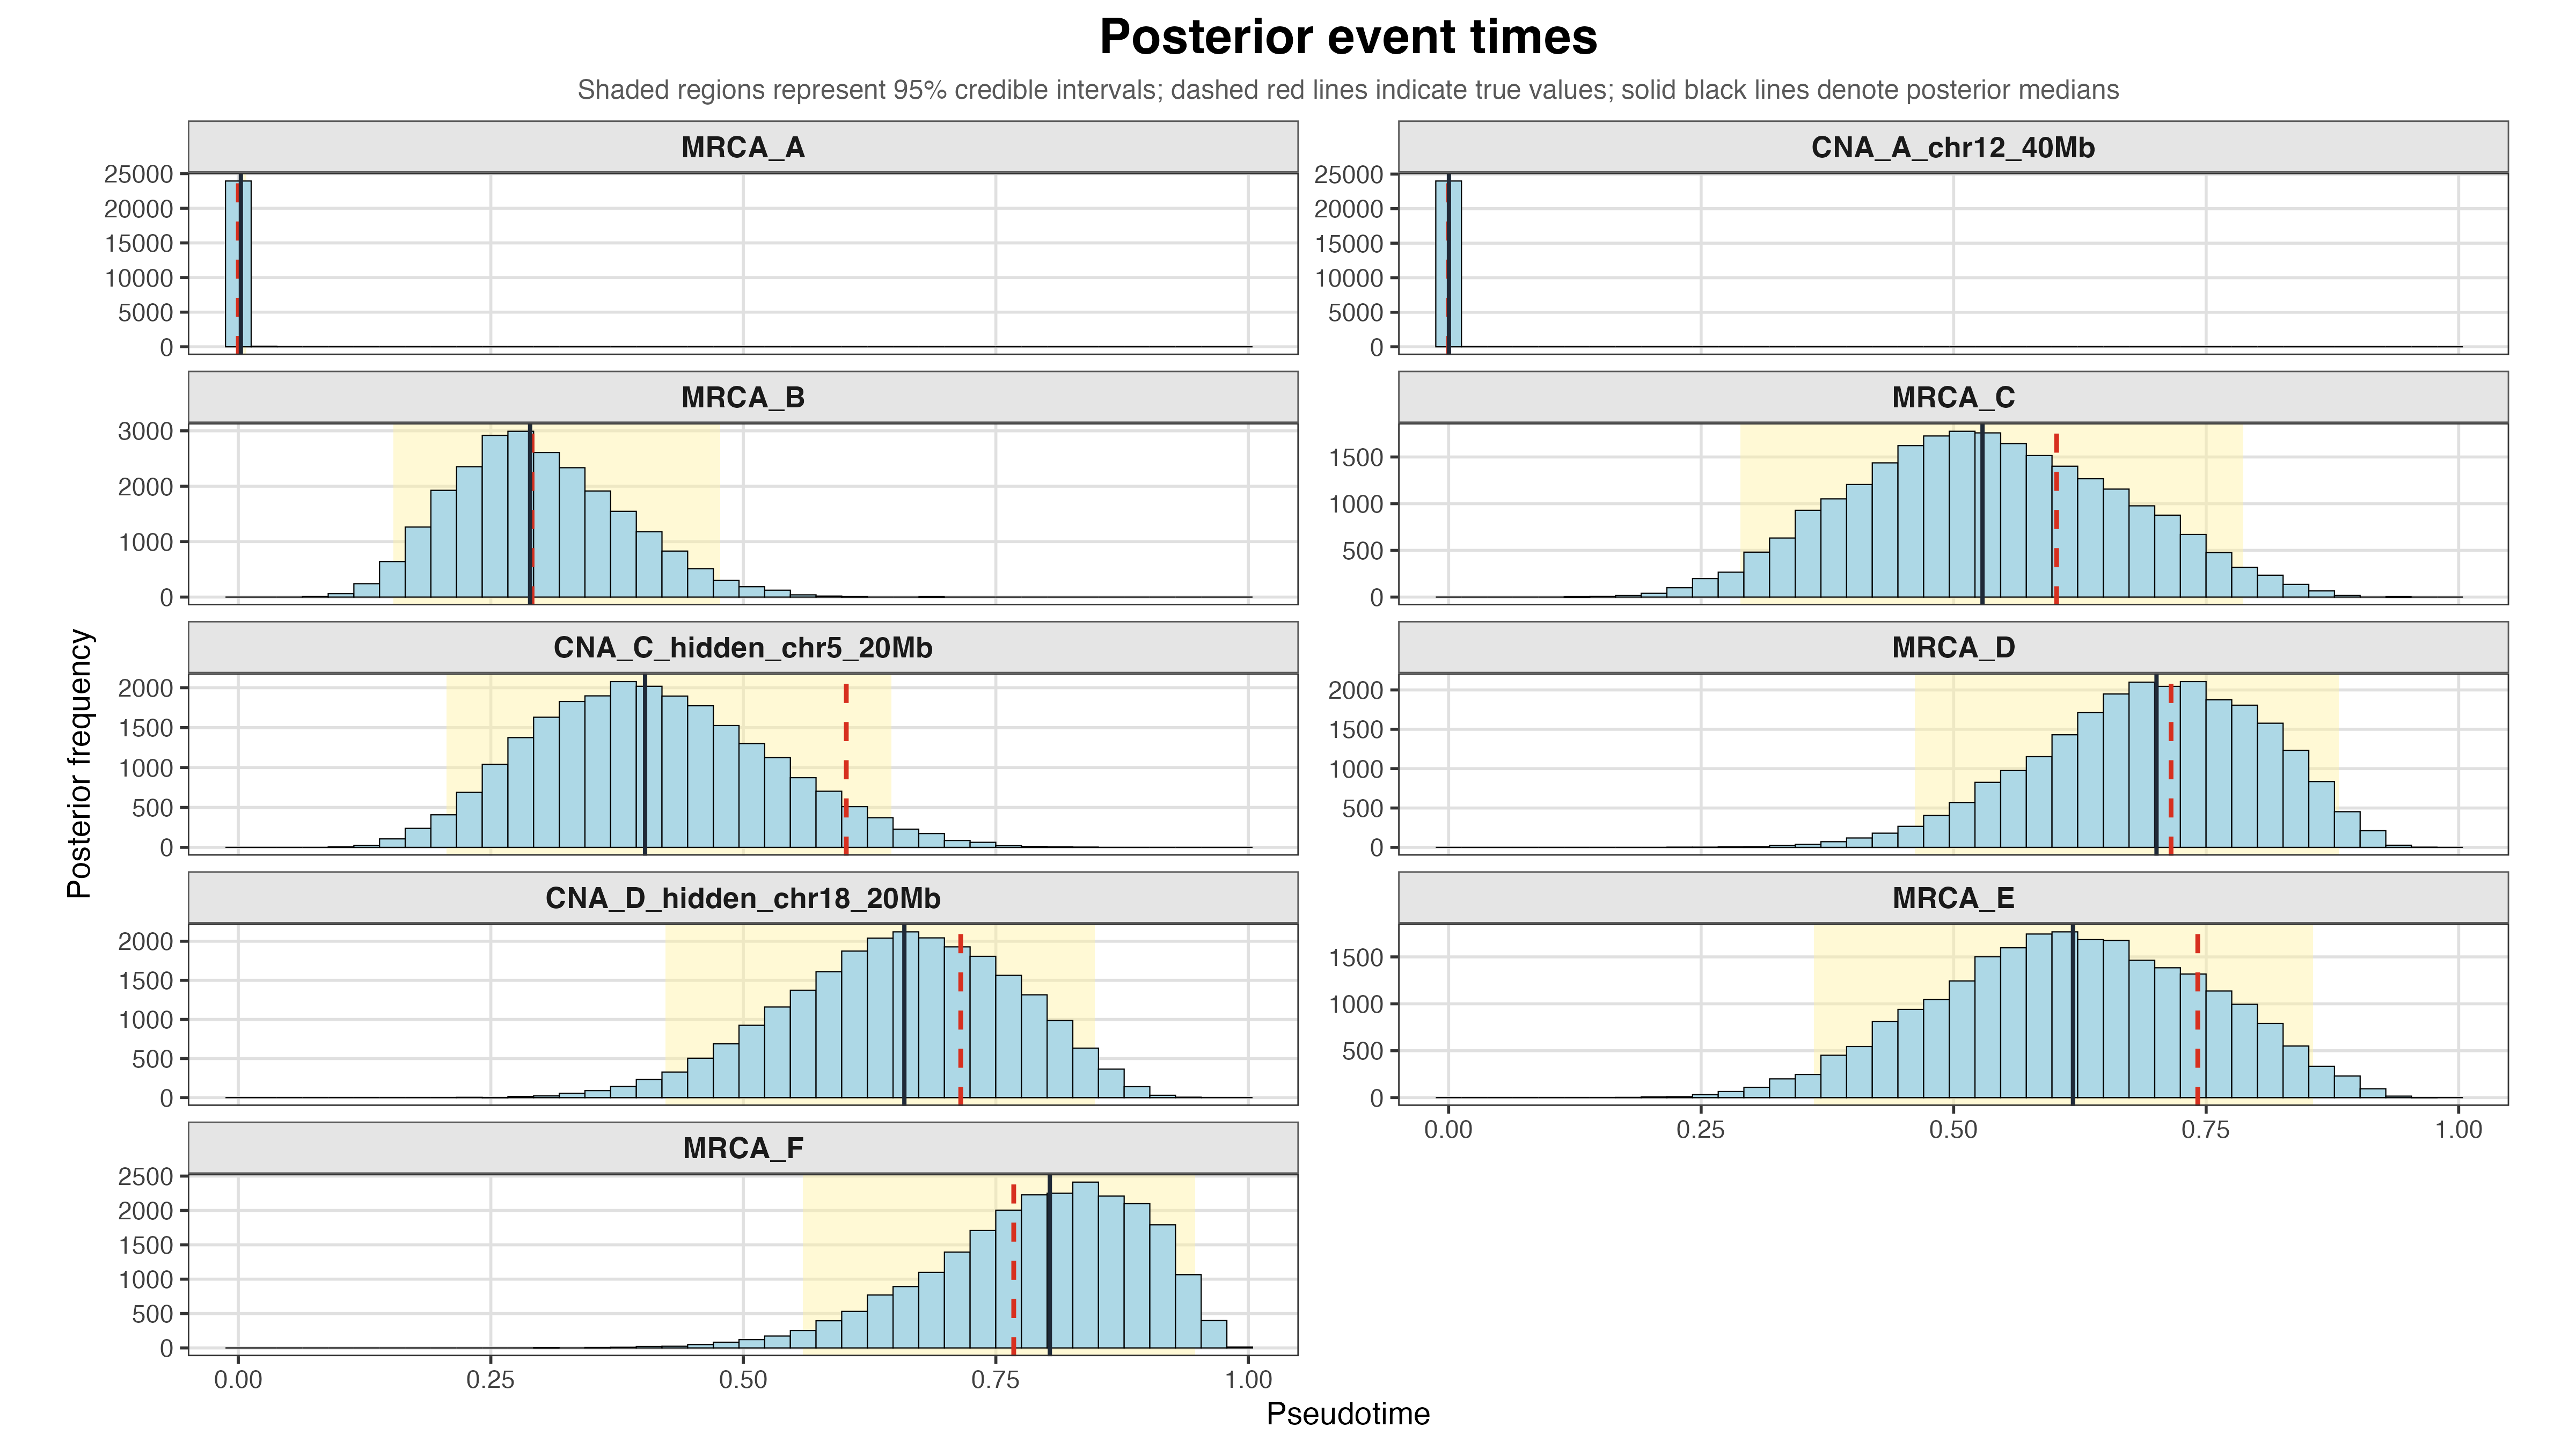
\includegraphics[width=0.8\linewidth]{immagini/figures 6 DLP/Posterior_Event_Times.png}
    \captionsetup{font=footnotesize}
    \caption{Posterior event pseudotimes for the six-clone scenario under localized
    biopsy sampling.}
    \label{fig:c6d-times}
\end{figure}

\begin{figure}[H]
    \centering
    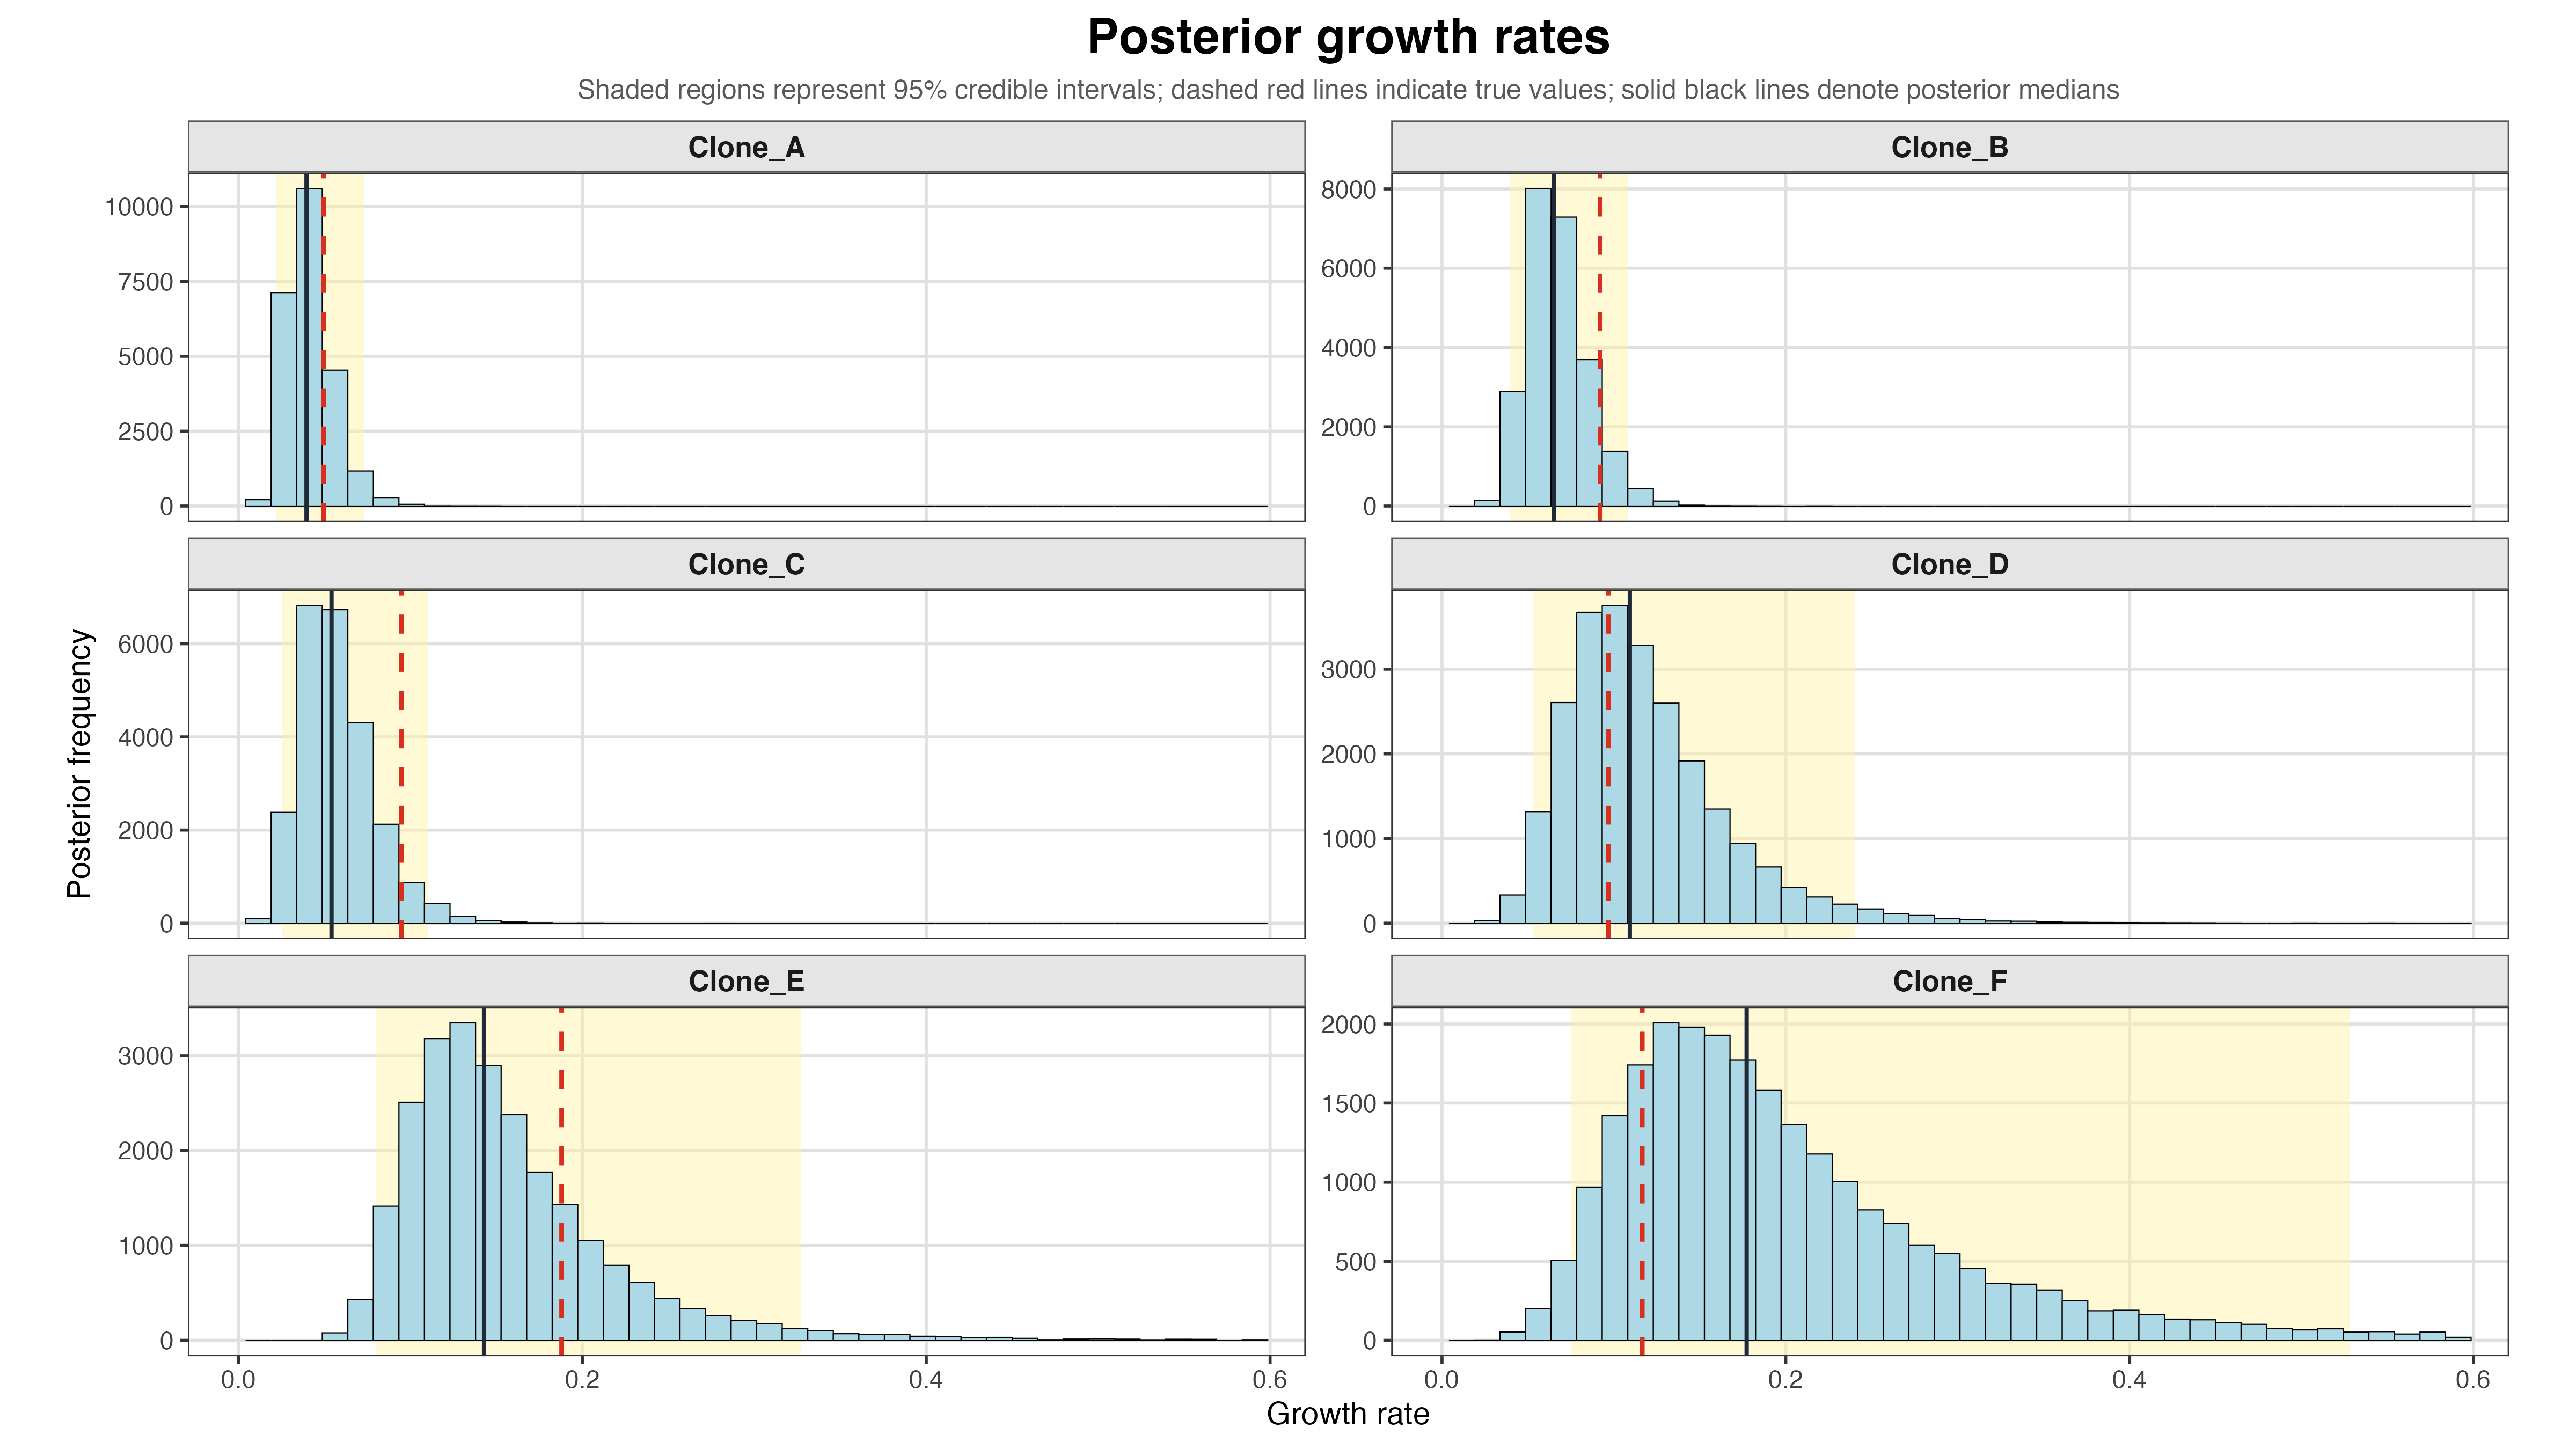
\includegraphics[width=0.8\linewidth]{immagini/figures 6 DLP/Posterior_Growth_Rates.png}
    \captionsetup{font=footnotesize}
    \caption{Posterior growth rates for the six-clone scenario under localized
    biopsy sampling; coverage is retained for all six clones.}
    \label{fig:c6d-growth}
\end{figure}

The mutation counts are reproduced on the harder tree too: the observed value lies
inside the $95\%$ posterior-predictive band for eleven of the twelve equations
(Figure~\ref{fig:c6d-mut-dist}). The lone exception is a low-count branch, where the
discreteness of small Poisson counts makes the interval narrow and a handful of
observed mutations sit just above a predictive distribution concentrated near zero;
the high-count branches, in the hundreds to nearly two thousand, are matched almost
exactly.

\begin{figure}[H]
    \centering
    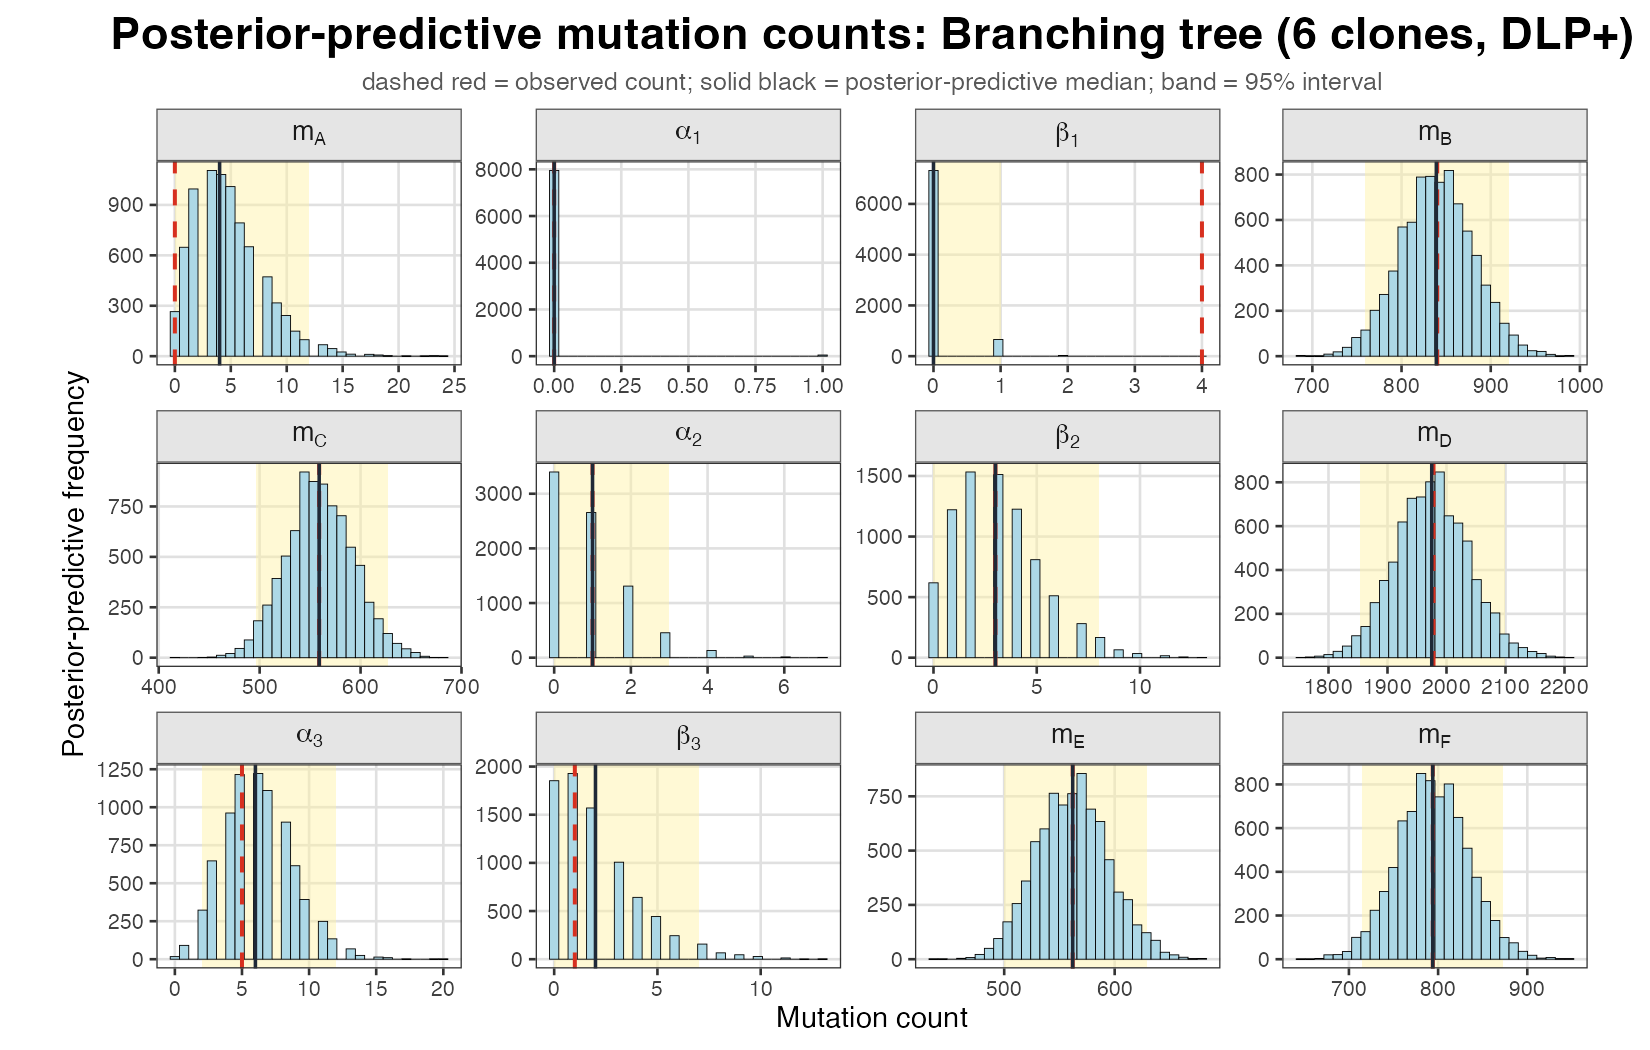
\includegraphics[width=\linewidth]{immagini/mut_dist_c6_dlp.png}
    \captionsetup{font=footnotesize}
    \caption{Per-equation posterior-predictive distribution of the mutation counts
    for the six-clone scenario under localized biopsy. Each panel is one mutation
    equation; the dashed red line is the observed count, the solid line the
    predictive median, and the band the $95\%$ predictive interval. Eleven of the
    twelve observed counts fall inside their intervals; the exception is the low-count
    branch (Eq~03).}
    \label{fig:c6d-mut-dist}
\end{figure}

The six-clone scenario splits the verdict: the event times and the mutation counts are
reproduced, while the growth rates lose precision though not calibration.

Table~\ref{tab:sim-bias} collects the recovery metrics for the two ProCESS scenarios,
reported separately for the event pseudotimes and the clone growth rates. Each block
holds three summaries, averaged over the events or clones of that scenario. The mean
absolute bias (MAB) is the average distance between the posterior median and the
truth, in the same units as the quantity (pseudotime on $[0,1]$ for the times, growth
units for the rates). The root-mean-square error (RMSE) is the square root of the
average squared error: it weights large misses more heavily than MAB, so a gap between
the two columns flags a few events estimated much worse than the rest. The median
relative bias (Rel.\ bias) is the typical \emph{signed} error as a fraction of the
true value, so its magnitude says how large the error is in relative terms and its
sign says whether the inference tends to over-estimate (positive) or under-estimate
(negative). Lower MAB and RMSE are better, and a relative bias near zero means no
systematic over- or under-estimation. The pseudotimes are on a common $[0,1]$ scale,
so their MAB and RMSE are directly comparable between the two scenarios.

% requires: \usepackage{booktabs}
\begin{table}[H]
\centering
\captionsetup{font=footnotesize}
\caption{Posterior bias of the inference for the two ProCESS scenarios, reported
separately for the event pseudotimes and the clone growth rates. MAB is the mean
absolute bias, RMSE the root-mean-square error, and Rel.\ bias the median relative
bias; all three are averaged over the events or clones of each scenario. Lower MAB
and RMSE are better, and the sign of the relative bias gives the direction of the
error.}
\label{tab:sim-bias}
\begin{tabular}{lcccccc}
\toprule
 & \multicolumn{3}{c}{Event pseudotime} & \multicolumn{3}{c}{Growth rate} \\
\cmidrule(lr){2-4}\cmidrule(lr){5-7}
Scenario & MAB & RMSE & Rel.\ bias & MAB & RMSE & Rel.\ bias \\
\midrule
Linear chain (4 clones)   & 0.020 & 0.024 & \phantom{-}0.001 & 0.025 & 0.038 & \phantom{-}0.108 \\
Branching tree (6 clones) & 0.056 & 0.085 & -0.078 & 0.033 & 0.037 & -0.220 \\
\bottomrule
\end{tabular}
\end{table}

The growth-rate columns make the pattern explicit: the median relative bias rises from
about $11\%$ on the four-clone chain to about $22\%$ on the deeper six-clone tree,
while the event-time error stays small ($\mathrm{MAB}\le 0.06$ in pseudotime) in both.
It is the depth of the phylogeny, not the way the tissue is sampled, that limits how
well the per-clone growth can be pinned down.

